%        File: memoria.tex
%     Created: sáb jun 28 01:00  2008 C
% Last Change: sáb jun 28 01:00  2008 C
%
\documentclass[a4paper,spanish,12pt]{book}
\title{BLAS: Base Layer for Application Services}
\author{Eduardo Orive Vinuesa}
\usepackage{babel}
\usepackage{times}
\usepackage[T1]{fontenc}
\usepackage[utf8]{inputenc}
\usepackage[left=2.5cm, right=2.5cm]{geometry}
\usepackage{a4}
\usepackage{makeidx}
\usepackage{graphicx}
\usepackage{float}
\usepackage{url}
\usepackage{setspace}
\onehalfspacing
\usepackage{fancyheadings}
\usepackage{wrapfig}
\usepackage{verbatim}
\usepackage{hyperref}
\usepackage{appendix}
\onehalfspacing

\begin{document}

%\maketitle
\begin{titlepage}
  \begin{center}
    \begin{tabular}[c]{c c}
      
\includegraphics[scale=0.5]{img/urjc.eps} &
      \begin{tabular}[b]{l}
        \Huge
        \textsf{UNIVERSIDAD} \\
        \Huge
        \textsf{REY JUAN CARLOS} \\
      \end{tabular}
      \\
    \end{tabular}

    \vspace{3cm}

    \Large
    INGENIERÍA INFORMÁTICA

    \vspace{0.4cm}
    
    \large
    Curso Académico 2007/2008
    
    \vspace{0.8cm}
    
    Proyecto Fin de Carrera
    
    \vspace{2.0cm}
    
    \LARGE
    BLAS:\\ BASE LAYER FOR APPLICATION SERVICES
    
    \vspace{3cm}
    
    \large
    Autor: Eduardo Orive Vinuesa \\
    Tutor: Gregorio Robles Martínez \\
    Co-tutor: Agustín Santos M\'endez 
  \end{center}
\end{titlepage}

\cleardoublepage
\thispagestyle{empty}
\vspace*{15cm}

\begin{flushright}
(c) 2008 Eduardo Orive Vinuesa


Este trabajo se entrega bajo licencia \\
Free Documentation License 1.2.\\
http://www.gnu.org/copyleft/fdl.html\\

Vea Apéndice para más detalles.
\end{flushright}

\pagenumbering{Roman}
%cuerpo del documento
\chapter*{Resumen}
BLAS es una plataforma pensada para orientar los esfuerzos dedicados a programar un servicio de internet, originalmente pensado para protocolos de tipo de texto sobre TCP/IP se ha extendido su funcionalidad a UDP/IP y en un futuro se proveera un soporte más fiable para protocolos binarios.

Con el objetivo de mejorar el proceso de diseño e implementación se aconseja organizar el proceso de atención de las peticiones en una serie discreta de estados lo más simples posible, estos estados se materializan en m\'etodos con nombres concretos que van dirigiendo la ejecución de uno a otro. Este modo de trabajo estructura y facilita de forma considerable el trabajo sobre protocolos con un formato concreto.

El desarrollo de servicios con este sistema provee de una estructura y permite acelerar el proceso de obtención de un prototipo estable.

La elección de Python como lenguaje permite una gran flexibilidad en la programación y sobretodo claridad en el código resultante. Precismante mantener la claridad en la implementación es una de las principales premisas a la hora de orientar la programación del servicio.

Se ha optado por la licencia GPL para proteger el proyecto y garantizar su disponibilidad futura, en especial a la comunidad de estudiantes y facilitar la participación a aquellos interesados en la platafoma y en el software libre.

\cleardoublepage


\pagestyle{plain}
\newpage
\tableofcontents
\newpage
\listoffigures
\cleardoublepage

\pagenumbering{arabic}

\pagestyle{fancyplain}


\chapter{Introducción}
Actualmente casi la totalidad de las instalaciones inform\'aticas son redes, y una mayoria de estas est\'an conectadas a Internet e incluso la propia Internet forma parte de estas.
\begin{figure}[h] %{r}{0.35\textwidth}
	\begin{center}
	\includegraphics[width=0.65\textwidth]{img/SistemasDistribuidos.eps}	
	\end{center}
	\caption{Ejemplo de un Sistema Distribuido}
	\label{fig:SistemasDistribuidos}
\end{figure}
\section{Historia de los servicios informáticos}
Despu\'es del desarrollo de la primera generación de computadoras el número de estas empezo a aumentar, aunque su disponibilidad estaba normalmente limitada a una unidad por cada entidad (instituciones educativas e instalaciones militares). Estas máquinas requerían de un entorno ambiental muy concreto y el acceso instalaciones donde se albergaban estaba severamente restringido. Por estas mismas limitaciones y para maximizar la disponibilidad se ideó un sistema limitado de terminales remotas, los teletipos, cuya funcion era comunicar con el ordenador central pudiendo utilizar enlaces dedicados o conmutados (lineas telefónicas), permitir la inserción de programas y recuperar el resultado una vez el sistema hubiera finalizado. Estos sistemas de comunicación y control remotos merecen la consideración de servicios informaticos.

Con el tiempo la versatilidad de los sistemas fue ampliandose, los ordenadores dejaron de emplearse como meras ejecutoras de algoritmos y empezaron a ofrecer distintos tipos de servicios:
\begin{enumerate}
	\item Boletines de noticias
	\item Transferencias de ficheros
	\item Correo electronico
\end{enumerate}
Es precisamente en esta \'epoca cuando empiezan implantarse sistemas de comunicacion por conmutacion convencionales y los servicios empiezan a emplear estos nuevos medios de enlace. La oferta de servicios deja de estar limitada a las grandes entidades y empiezan a surgir ``BBSes'' (Bulletin Board System) albergadas en ordenadores privados. Durante más de 25 años han sido un medio de comunicación y entretenimiento, en opinión de muchos sigue siendo los mejores ambientes comunitarios. 

La capacidad monousuario de los sistemas de la epoca presento la necesidad de empezar a dejar de utilizar enlaces de lineas conmutadas para añadir un nuevo nivel de paquetes conmutados para eliminar esta limitación.

Con el tiempo y con el inexorable cumplimiento de la ley de moore, los sistemas fueron ampliando geometricamente su capacidad, tambien lo hacia su disponibilidad en el mercado haciendose cada vez asequibles para el público en general, acompañado por una reducción drástica del volumen y consumo energ\'etico.  

La popularización de internet llevó a que practicamente cualquier ordenador dom\'estico estuviera dotado de algún dispositivo de comunicación metropolitana y una pila IP, permitiendo así acceder a los servicios ofrecidos en internet a trav\'es del respetivo ISP. 

En poco tiempo dispositivos portatiles imitaban la tendencia junto a otros microdispositos. Es muy común ver que aparatos convencionales, desde electrodomesticos a vehiculos lleven incorporados sistemas de comunicación que automáticamente son capaces de desempeñar tareas como emitir a la central la posición del vehículo y todo tipo de medidas cuatificables sobre su estado. 

\section{Motivación}

En los último años cursando Ingeniería Informática y en proyectos profesionales se ha presentado en numerosas ocasiones la necesidad de escribir servicios orientados a internet. La necesidad de encontrar un sistema estruturado y rapido de elaboración de prototipos es lo que ha inspirado la creación de esta plataforma.

Es en este entorno donde se desarrollan las arquitecturas de la mayor\'ia de los sistemas. Distribuidas y en una gran proporci\'on siguiendo el modelo Cliente-Servidor casi todas las nuevas aplicaciones o sistemas basan gran parte de su funcionalidad en la conectividad mediante redes. 

Sin embargo realizar aunque sea un prototipo operativo de un servicio de red requiere de una importante inversion en tiempo y no se obtienen resultados tangibles hasta que se ha implementado una buena parte del código.
Tambi\'en muy com\'un ver que muchos prototipos sean descartados (total o parcialmente) y deban re-implementarse ya que, aunque su rendimiento sea aceptable, la seguridad que ofrecen no lo es, con lo que el proceso de crear el servicio duplica su coste cuando el sistema llega a la etapa de producci\'on.

No obstante la escritura de un servicio de Red puede reducirse considerablemente si se implementan tan solo las caracteristicas particulares de su protocolo. Basicamente cualquier protocolo puede entenderse como un automata m\'as o menos complejo, siguiendo este modo de dise\~{o} puede simplificarse de manera considerable el trabajo del programador.

La intención principal de esta plataforma es evitar la reimplementación innecesaria de funcionalidades que son comunes a todo tipo de servicio de red interactivo, además de proponer una metodología concreta en la implementación.
\section{Disponibilidad del proyecto}
Este proyecto se ha traspasado desde una de sus mas primitivas versiones al repositorio que google dispone para desarrolladores. La elección de \url{http://code.google.com/} como repositorio se ha debido sobre todo al electo de herramientas y servicios que Google está dedicando a los desarrolladores de software y sobre todo a los proyectos de programación colaborativos.

Todo el código y la documentación referente a este proyecto podrá encontrarse en \url{http://code.google.com/p/blas/}. La participación de terceros quedará abierta en cuanto se evalue el proyecto, en mi opinión ese será el verdadero comienzo de la plataforma, cuando se pruebe su uso y las aportaciones de otros desarrolladores amplien sus funcionalidades.
\section{Licencias}
Este proyecto dispone de 2 licencias: una para el propio software que garantice a futuros la disponibilidad de este para toda la comunidad de software libre, otra para este documento, de tal forma que su contenido pueda aprovecharse en otros esfuerzos de documentación colaborativa como \url{http://es.wikipedia.org}.

Ambos documentos pueden encontrarse en la sección de anexos.
\chapter{Objetivos}

Esta plataforma se ha ideado para facilitar el diseño y la implementación a los colectivos que por diversos motivos se ven ante la necesidad de programar un servicio de red en poco tiempo. 

Existen multitud de funcionalidades ligadas a los programas que ofrecen servicios TCP y UDP, que inevitablemente consumen mucho tiempo y que normalmente los programadores se encuentran realizando funciones de implementación muy similares de un proyecto a otro pero sin permitir una reutilización eficiente del código.

Básicamente estas tareas se reducen a:
\begin{enumerate}
	\item Entrada controlada de datos.
	\item Registro (o registros) de actividad y error.
	\item Lectura de los archivos de configuraci\'on.
	\item Parseado de los parametros de arraque.
\end{enumerate}

El objetivo principal de esta librería es facilitar las tareas de diseño e implementación de este tipo de software. Acelerando la aparición de prototipos que permitan iniciar lo antes posible la depuración tanto del servicio como de los clientes.

Es posible que existan dudas sobre si actualmente existe la necesidad de la realizacion de este tipo de software. Hoy día se pueden encontrar cientos de implementaciones de protocolos sobre multitud de tecnologías diferentes existe todavía la necesidad de realizar implementaciones de servicios de protocolos antiguos o nuevos.

\section{Docencia}
Existen numerosos proyectos academicos que requieren la implementaci\'on de:
\begin{enumerate}
	\item Protocolos nuevos,
	\item Protocolos ya existentes.
	\item Modificaciones sobre protocolos antiguos. 
\end{enumerate}

y que pueden ver facilitada su realización utilizando esta plataforma.

\section{Microdispositivos}
La mayor\'ia de los dispositivos dotados de un sistema operativo m\'inimo disponen de una modesta pila IP ya que, practicamente todos estos dispositivos, se dise\~{n}an incluyendo algún tipo de hardware de interconexi\'on mediante enlaces de radio o cableado . Sin embargo por razones de coste economico y rendimiento energetico se ven afectados por una leve capacidad de memoria y/o potencia de c\'alculo que hacen que la opcion de conectarlos a un servicio convencional (HTTP y REST por ejemplo) resulte muy engorrosa (y caro) en su programaci\'on, e incluso a veces impracticable.

Es por este motivo que se suelen dise\~{n}ar protocolos normalmente muy escuetos, especificamente adaptados a la funcionalidad del dispositivo y a sus limitaciones de proceso.

\section{Seguridad Inform\'atica}
En un entorno en que los ataques mediante gusanos son casi rutinarios se emplea mucho tiempo y esfuerzo en crear servicios que se comporten como los originales que emplee el gusano para penetrar en el sistema y as\'i poder estudiar que acciones realiza una vez dentro.

La capacidad de programar servicios simulados agilmente puede ser un complemento perfecto a otras herramientas de estudio de la seguridad como son las 'Honey-Nets', dotando a las m\'aquinas virtuales de un comportamiento mucho m\'as flexible.



\chapter{Estado del arte}

\section{Lenguaje: Python}
\subsection{Elecci\'on del Lenguaje} 
Se ha elegido Python como lenguaje de programaci\'on para esta plataforma por las siguientes razones:
\begin{enumerate}
	\item Velocidad de aprendizaje: cualquier persona que conozca un lenguaje orientado a objetos puede aprenderlo en muy poco tiempo.
	\item Reflexividad e introspección: Las clases en pytohn tienen conocimiento de sus propios metodos y atributos.
	\item Interpretado: Al ejecutarse bajo un interprete no har\'an falta compilar distintos ejecutables seg\'un la plataforma.
\end{enumerate}

Con el empleo de Python se puede conseguir con pocas lineas la implementaci\'on de un protocolo completo. Al tratarse de un lenguaje en que la identaci\'on es obligatoria y la sintaxis muy clara normalmente su codigo fuente esta bien estructurado y resulta facil de leer incluso para quienes apenas conozcan Python.

\subsection{Python: historia y características}

Python fue creado como sucesor del lenguaje ABC por Guido van Rossum en 1990 cuando trabajaba en el Stichting Mathematisch Centrum (CWI). En 1995 Guido continuó su trabajo en Python en el CNRI donde creó muchas versiones del lenguaje. En mayo del 2000 Guido y el equipo de desarrollo de Python se trasladan a BeOpen.com y se forma el BeOpen PythonLabs. En octubre de este mismo año, PythonLabs se va a Digital Creations (actualmente Zope Corporation). En 2001, se crea la Python Software Foundation (PSF), una organización sin ánimo de lucro creada específicamente para proteger la libertad de Python como lenguaje de código abierto.

El nombre del lenguaje proviene de la afición de su creador original, Guido van Rossum, por los geniales humoristas británicos Monty Python.

Python ha sido usado para crear programas tan famosos como el gestor de listas de correo Mailman o los gestores de contenido Zope y Plone.

Python se puede encontrarse en varias encarnaciones. En el sitio web de la Python Software Foundation, Python esta implementado en C. Pero existen otras: Basada en Java una implementacion denominada Jython puede utilizarse para trabajar con codigo Java nativamente. Iron Python, una version en C\# existe para hacer uso de las plataformas Mono y .Net y que los programadores de estas puedan beneficiarse de su potencia y flexibilidad. En cada una de estas encarnaciones Python se ha escrito en un lenguaje y funciona nativamente en este aunque puede tambien intectuar perfectamente con otros lenguajes a trav\'es de sus correspondientes modulos.

Con propositos de investigacion y desarrollo existe tambi\'en una implementacion de Python sobre Python. El proyecto PyPy fue iniciado en 2003 con la intencion de permitir a los programadores en Python modificar el comportamiento del interprete. Además se trata de un proyecto de codigo abierto, desarrollado por una comunidad para libre distribución y modificacion, PyPy está patrocinado por la Unión Europea como un STReP (Specified Targeted Research Project), parte del plan de apoyo FP6.

\subsection{Evolución}

\subsubsection{Primera publicación}

En 1991 van Rossun puclido el codigo (con la versión 0.9.0) en alt.sources. Ya en este primer estado de desarrollo habia clases con herencias, manejo de expeciones, funciones y los tipos de datos basicos de listas, diccionarios, cadenas y demás. Tambi\'en en esta publicación inicial habian un modulo de sistema que fue tomado prestado de modula3; van Rossum define este modulo como ``una de las principales unidades de programación de Python''. El modelo de gestión de excepciones de python tambi\'en imita al de Modula3 salvo que incluye la clausula ``else''. En 1994 arranca comp.lang.python, la primera lista de discussion de python, marcando un hito en el crecimiento de la base de usuarios de Python.

\subsubsection{Version 1.0}

Python llego a la version 1.0 en Enero de 1994. Las principales nuevas funcionalidades incluidas en esta publicación fueron las utilidades de programación funcional lambda, map, filter y reduce. Van Rossum expreso que ``Python a conseguido lambda, reduce, filter y map por cortesia (en mi opinión) de algun hacker de Lisp que las echabada de menos y envio parches operativos''.

La ultima version publicada cuando van Rossun estaba en el CWI fue Python 1.2. En 1995 van Rossum continuó su trabajo en la Corporacion para Iniciativas de Desarrollo Nacional (CNRI) en Reston (Virginia) desde la que publicó varias versiones.

Por la version 1.4, Python habia conseguido varias nuevas funciones. Es de destacar que entre estas son los parametros por palabra clave de Modula3 (Que son tambien similares a los parametros por palabra clave de Lisp) y el soporte integrado para números complejos. Tambin incluye una forma basica de ocultamiento de datos por manipulacion de nombre, aunque podia ser facilmente obviado.

Durante la estancia de var Rossum en el CNRI, lanzo la iniciativa Programacion de Ordenadores para Todos (CP4E), que pretendia hacer la programacion mas accesible a mas gente, con un conocimiento basico en lenguajes de programacion, de forma similar a los conocimientos basicos de literatura inglesa y matematicas que se exigen a cualquier empleado. Python sirvio con un papel central en esto: devido a su enfoque en una sintaxis clara, ya podia considerarse adecuado, y los objetivos del CP4E ya apuntaba parecidos con su predecesor ABC. El proyecto fue fundado por DARPA. En 2007 el proyecto parece inactivo y aunque Python pretende ser de facil aprendizaje y no demasiado arcano en su sintaxis y semantica, llegar a ser comprensible para los no programadores no es una intencion activa.

\subsubsection{Version 2.0}

Python 2.0 introdujo la comprensión de listas, una funcion prestada de los lenguajes de programacion funcionales Lips y Haskell. La sintaxis de python en su construccion es muy parecida a la de Haskell, dejando a un lado la preferencia de Haskell por los caracteres de puntuacion y la preferencia de Python por las palabras clave alfabeticas. Python 2.0 tambien introdujo un sistema de recoleccion de basura capaz de tratar referencias ciclicas.

Python 2.1 era bastante parecido a Python 1.6.1, al igual que Python 2.0. La licencia cambio su nombre a Python Software Foundation License. Todo el codigo, documentacion y especificaciones añadidas, desde la alpha de Python 2.1, es propiedad de la Python Software Foundation, una organizacion sin animo de lucro formada en 2001, modelada siguiendo el ejemplo de la Apache Software Foundation. La publicación incluyó un cambio en la especificacion del lenguaje para soportar intervalos (scopes) anidados, al igual que otros lenguajes con intervalos estáticos. Esta función estaría desactivada por defecto y no fue necesaria hasta Python 2.2.

Una de las principales innovaciones en Python 2.2 fue la unificacion de los tipos de Python (tipos escritos en C) y clases (tipos escritos en Python) en una unica jerarquía. Esta unificacion hizo al modelo de objetos de python un modelo orientado pura y consistentemente a objetos. Tambi\'en se añadieron generadores inspiradores por el lenguajes Icon.

\subsubsection{Version 2.6}

En el momento de desarrollar esta librería, python 2.5 y python 3.0 conviven en muchos proyectos, sin embargo y aunque se pueda ejecutar sobre 3.0, el poco tiempo que lleva la versión 3.0 en funcionamiento hace poco recomendable su utilización en sistemas que requieran de una cierta estabilidad.

\subsubsection{Disponibilidad}

En muchos sistemas operativos Python es un componente estandar, se incluye en la mayoria de las distribuciones de Linux, NetBSD, OpenBSD y con Mac OS X. Slackware, Red Hat Linux y Fedora utilizan el instalador Anaconda, escrito en Python. Gentoo Linux utiliza Python en su sistema de administración de paquetes Portage, y su herramienta por defecto Emerge. Pardus lo utiliza para administración y durante el arranque del sistema.

\subsubsection{Editores}

Python puede programarse con cualquier tipo de editor y siempre permitirá una lectura clara y una estructura adecuada del código. Sin embargo son muchos los editores y entornos integrados de trabajo que incluyen funciones de ayuda en la programacion:
\begin{enumerate}
	\item{Resaltado del código: Cualquier editor con unas funcionalidades de programación minima incluirá resaltado de sintaxis.}
	\item{Prediccion de escritura: Prácticamente cualquier editor incluirá indentación automatica y probablemente predicción de palabras clave.}
	\item{Gestión de proyectos: Disponible sobre todo en IDEs y raramente en editores.}
	\item{Shell integrada: Disponible en algunos de los editores y la mayoría de los IDEs.}
\end{enumerate}

Para conseguir una lista actualizada de editores compatibles con python en todas las plataformas puede conseguirse en esta URL: 
http://wiki.python.org/moin/PythonEditors


\section{Protocolos de red: IP}
Es dificil generalizar sobre protocolos ya que estos varian ampliamente en proposito y en complejidad. La mayoria de los protocolos de red poseen alguna de las siguiente propiedades:

\begin{wrapfigure}{r}{0.35\textwidth}
	%{figure}[h]
	\includegraphics[width=0.25\textwidth]{img/NivelesOSIRed.eps}	
              \caption{Niveles OSI: protocolo de red}
  \label{fig:nivelesOSIRed}
\end{wrapfigure}


\begin{enumerate}
\item Detección de la capa subyacente de enlace de red, o la existencia de otro punto de entrada o nodo.
\item Saludo y reconocimiento (Handshaking)
\item Negociación de varias de las caracteristicas de la conexión.
\item Como indicar el comienzo y el final de un mensaje.
\item Formato de los mensajes.
\item Como actuar ante mensajes corruptos o con un formato incorrecto (corrección de errores)
\item Como detectar una perdida inesperada de la conexion y como comportarse ante esta.
\item Finalizar la sesión o conexión.
\end{enumerate}

En concreto el protocolo de Internet (IP) se utiliza en los extremos de la comunicación para mantener un flujo de datos a traves de una red de paquetes coonmutados.

Precismente debido a la naturaleza de estas redes los datos son divididos en cantidades coherentes a las limitaciones del medio (por ejemplo 1500 bytes para redes ethernet), estos fragmentos de información se les denominan paquetes o datagramas. Además el protocolo no requiere que las rutas que deben seguir estos paquetes sean establecidas de antemano, es el propio protocolo el que encontrará la ruta idonea.

Con el protocolo IP se provee un sistema para la transmision de datagramas no fiable (best effort), este metodo de transmisión no garantiza resultados pero intentará utilizar la ruta más efectica. Debe aclararse que IP no posee mecanismos para garantizar que la transmisión ha llegado a destino, aunque si dispone de mecanismos para la detección de errores en los datos que contenga el paquete. Debido a la naturaleza dinámica de las rutas y a la hetereogeneidad de los dispositivos es probable que los datagramas en que ha sido dividido el flujo de datos lleguen fuera de orden e incluso que llegue repetido, es tarea de los protocolos de transporte detectar estos sucesos.

A lo largo de la ruta es posible que la longitud maxima de transmision (MTU) vaya cambiando (por ejemplo de 1500bytes de ethernet a 576 de una conexion punto a punto). Es tarea del protocolo IP volver a fragmentar estos datagramas en otros más pequeños y recomponerlos cuando sea necesario, debe tenerse en cuenta que estos fragmentos pueden utilizar vias diferentes en según que tramos de la ruta.

Para manejar estos incidentes el protocolo acompaña a las tramas de datos en los datagramas de una cabeceras, estas llevan incluidas las direcciones IP del origen y destino de la comunicacion, estas son requeridas por los dispositivos que retransmitirán los datos a trav\'es de las rutas para seleccionar el camino adecuado.

Actualmente el protocolo mas utilizado en Internet es el IP version 4 (IPv4 en adelante). Sin embargo ya se ha propuesto un sucesor, IPv6, llamado a eliminar las limitaciones que afectan a IPv4 desde su diseño. Una de estas nuevas caracterisiticas es el empleo de direcciones de 128bits, que permitiria otorgar una dirección univoca a mas de 670 mil millones de dispositivos. 

Cabe señalar las las versiones 0 a la 3 del protocolo IP no llegaron a emplearse  y que la version 5 se utilizó para un prototipo experimental. Además IPv4 dispone de diferentes implementaciones que buscan mejorar su eficiencia o limitar el efecto de sus deficiencias.

\section{Protocolos de transporte}

Basandonse en el nivel de Red (lo que proporciona una ruta de comunicación y un medio libre de errores inesperado en los datos recibidos) existe un nuevo nivel OSI. Los protocolos de este nivel tienen la responsabilidad de controlar la entrega en destino de los datos y en la medida de lo posible conseguirlo con una cantidad mínima de redundancia de datos.

\begin{wrapfigure}{l}{0.35\textwidth}
	\includegraphics[width=0.25\textwidth]{img/NivelesOSITransporte.eps}	
              \caption{Niveles OSI: protocolos de transporte}
  \label{fig:nivelesOSITransporte}
\end{wrapfigure}

Basandonos en esta jerarquía y situandonos sobre el protocolo de transporte los extremos de comunicación pueden dar las siguientes caracterisiticas por garantizadas :
\begin{enumerate}
	\item{Garantizar una transferencia libre de datos entre los interlocutores}
	\item{Mantener una ruta de comunicacion entre puntos que no est\'en directamente conexionados}
	\item{Control de flujo y gestión del buffer}
	\item{Multiplexión de las vias de comunicación}
	\item{Recuperación y redirección}
\end{enumerate}
\subsection{Protocolo TCP}
El Transfer Control Protocol es el encargado de proporcionar un medio de comunicación orientado a conexión. Permite controlar que los mensajes llegan de un extremo a otro en el orden correspondiente. Además detecta y según el caso corrige fallos en la conexión, ya sean errores en los mensajes recibidos, perdidas de tramas enteras o errores en parte de estas.

Las aplicaciónes sobre TCP envian y reciben flujos de datos de forma transparente (salvo error) a la aplicación que las utiliza, es el propio protocolo quien fragmenta la tramisión según los requisitos del medio y organiza que la recomposición de los datos sea coherente sea cual sea el orden de llegada.

Las cabeceras del protocolo TCP son bastante complejas

Los programas que utilizan una conexion TCP para transmitir datos lo hacen de manera transparente, envian el flujo de bytes y es el protocolo el que la divide en paquetes según la configuración de la capa de red, adjunta ademas su propia cabecera, que será indispensable para conseguir una recepción coherente de los datos, ya que incluye entre otros campos el número de secuencia. Durante la operación una pila TCP va recibiendo los paquetes desde la capa IP, los ordena y organiza segun el número de secuencia. Para detectar la falta de paquetes y repetir la transferencia existe un mecanismo de asentimiento de la trasmisión: en la cabecera, un campo NACK indica al emisor de la información hasta que número de secuencia se han recibido todos los paquetes y se ha recompuesto los datos. El mecasnismo de caducidad (timeout) se activará si en un cierto tiempo el emisor no ha recibido confirmación por parte del receptor.
\begin{figure}[h]
	\begin{center}
	\includegraphics[width=0.90\textwidth]{img/CabeceraTCP.eps}	
\end{center}
\caption{TCP: Diagrama de cabecera}
  \label{fig:CabeceraTCP}
\end{figure}

A continuación se desglosan los campos contenidos en las cabeceras:
\begin{enumerate}
	\item{Puertos de origen y destino: identifica a que puerto de los extremos debe dirigirse el paquete}
	\item{Número de secuencia: Sirve para garantizar la coherencia y completud del flujo de datos que se esta enviando. Dependiendo de si el flag SYN esta o no activado puede indicarnos si ese número de secuencia será el inicial para esa transferencia de datos o si esta desactivado marcará el numero de secuencia del primer byte de datos.}
	\item{NACK: si el paquete es de tipo ACK entonces el receptor esta esperando que el siguiente paquete recibido sea el correspondiente al siguiente numero de secuencia.}
	\item{Longitud de cabecera: Especifica el tamaño de la cabecera en divisores de 32bits. A este campo tambien se le denomina dataoffset por ser eldesplazamiento necesario para acceder a la trama de datos.}
	\item{Reservado: estos bits deberán dejarse a 0, están reservados para aplicaciones futuras del protocolo.}
	\item{Flags: estos 8 bits de control se utilizan para regular el funcionamiento del protocolo:
		\begin{enumerate}
			\item{CWR: Congestion Window Reduced, avisa al receptor de que se esta produciendo congestion en la red y debe negociarse una reducción de la ventana del buffer.}
			\item{ECN-Echo: Se avisa al destino que puede emitir notificaciones ECN, este flag se usa durante la etapa de saludo.}
			\item{URG: Urgente, avisa de que el paquete debe ser tratado con prioridad en la pila}
			\item{PSH: Push, hace que los datos almacenados en el buffer sean traspasado a la aplicación}
			\item{ACK: Acknowlegde, hace que el número de acuse de recibo sea considerado por el receptor.}
			\item{RST: Reset, reinicializa la conexión}
			\item{SYN: Synchronize, obliga a que los numeros de secuencia est\'en sincronizados.}
			\item{FIN: Comunica el final del flujo de datos.}
		\end{enumerate}
	}
	\item{Ventana: es la capacidad de la ventana de recepcion, indica en bytes la cantidad de datos que el receptor esta esperando.}
	\item{Checksun: suma de comprobación que abarca tanto cabecera como datos.}
	\item{Urgente: Si esta el flag URG activado indica el offset respecto del número de secuencia del ultimo byte que debe considerarse urgente}
	\item{Opciones: Campo de información ajena al contenido de los datos, debe ser multimo de 32bits}
	\item{Datos: trama con el segmento de datos que se espera en el destino.}
\end{enumerate}

\subsubsection{Funcionamiento}
El protocolo TCP basa su funcionamiento en una serie de procedimientos consecutivos:
\begin{enumerate}
	\item{Saludo o establecimiento de la conexión: Consistente en la negociación de 3 pasos en la que tambi\'en se establecen los parametros clave de esta.}
	\item{Transferencia de los datos: en la que se van emitiendo asentimientos para confirmar la llegada de grupos de tramas}
	\item{Desconexión: para la que se procede a una negociación de 4 pasos}
\end{enumerate}

\begin{wrapfigure}{r}{0.45\textwidth}
	\includegraphics[width=0.35\textwidth]{img/TCPSaludo.eps}	
              \caption{Protocolo TCP: secuencia de saludo}
  \label{fig:TCPSaludo}
\end{wrapfigure}

Habitualmente para iniciar una conexión TCP un dispositivo cliente se comunica con un dispositivo servidor, que se encuentra escuchando en un puerto TCP concreto a traves de la pila IP. Antes de que tanto el cliente como el servidor dispongan de un socke se realiza una negociación de 3 pasos. El cliente emite un paquete SYN al puerto especifico del servidor, ahí el sistema operativo enviará la información al software que haya realizado el bind() a ese puerto. Si no existe ningún software escuchando se emitirá un paquete RST al cliente para que conozca el fallo de la operación. Si se ha alcanzado un puerto abierto el sistema responderá con un paquete SYN+ACK y para dar por establecida la conexión el cliente responderá a su vez con un paquete ACK. Es en este proceso cuando se elige al azar un número de secuencia que permitirá proceder correctamente en las operaciones de transferencia de datos.


Una vez establecida la conexión cliente y servidor dispondrán de un mecanismo de intercambio de datos muy similar al que se dispone cuando se abre un dispositivo de tipo caracter, el nivel de aplicación emitirá y recibirá datos de forma transparente y serán las capas de Trasnporte y Control las encargadas de que lleguen y se ordenen correctamente en destino.


El proceso de envio de datos requiere que se hayan determinado dos parametros clave obligatorios en el establecimiento:
\begin{enumerate}
	\item{Número de secuencia: que corresponderá al primer byte de la trama contenida en el paquete y que se espera en el otro extremoi. Cabe destacar que el numero de secuencia volver a 0 cuando haya sobrepasado el máximo}
	\item{Tamaño de ventana: es la cantidad de datos que pueden enviarse desde el emisor sin haber recibido confirmación de receptor.}
\end{enumerate}

Durante la transferencia el emisor envía un número de paquetes, este número depende del número de asentimiento (que es el número de secuencia reconocido por el receptor), el número de secuencia de los paquetes que esta enviando y la capacidad de la ventana de transferencia.

Normalmente el cliente ira recibiendo con un cierto orden los paquetes y modificando su propio número de secuencia. Periodicamente se informará al emisor con un paquete ACK del número de secuencia confirmado, mientras tanto, este reenviará el conjunto de paquetes que correspondan a la ventana actual. Tambi\'en se emitirán ACKs cuando el paquete que se ha recibido complete a un conjunto.

En ciertas implementaciones de TCP puede encontrarse una nueva función, el asentimiento selectivo, que permite avisar al emisor de que paquetes son necesarios para completar el conjunto actual indicando cuales se han recibido.

Uno de los motivos más comunes de la perdida de paquetes es la saturación del canal, se emiten más información de la que este puede enviar, con lo que los paquetes empiezan a ser descartados. Por este motivo TCP ha implementado sistemas para la detección de la saturación del canal, que regulan de una forma efectiva el tamaño de la ventana y el ritmo de emision de los paquetes.

\begin{wrapfigure}{l}{0.45\textwidth}
	\includegraphics[width=0.35\textwidth]{img/TCPDespedida.eps}	
              \caption{Protocolo TCP: secuencia de desconexión}
  \label{fig:TCPDespedida}
\end{wrapfigure}


Durante la finalización de una conexión uno de los extremos emite un paqute FIN, la respuesta consiste en dos paquetes, un ACK y posteriormente un FIN, cuando el emisor de la despedida emita un ACK la conexión se dará por concluida.

\subsubsection{Evolución}

\subsection{Protocolo UDP}

De entre los protocolos de transporte sobre IP, el User Datagram Protocol (UDP) es el mas básico de todos.

Orientado al simple envio de mensajes UDP ofrece un metodo de operacion muy sencillo para el acceso al protocolo de red. Sin embargo UDP no garantiza la recepcion del mensaje, con lo que el origen de los datos no tiene forma de saber mediante el propio protocolo en que estado se encuentra la transacción de datos, ni incluso si estos han salido a la red. Lo que si garantiza UDP es el multiplexado, la verificacion de errores y una minima proporcion del tamaño de la cabecera respecto de la trama util. 

Sin embargo si se desea obtener algun mecanismo para el control de la entrega de mensajes debe implementarse a nivel de aplicación.
\begin{figure}[h]
	\begin{center}
	\includegraphics[width=0.55\textwidth]{img/CabeceraUDP.eps}	
\end{center}
\caption{UDP: Diagrama de cabecera}
  \label{fig:CabeceraUDP}
\end{figure}

En su cabecera UDP solo necesita de 2 campos obligatorios y otros 2 opcionales (con letras grises en el diagrama). Cada uno de estos datos ocupan 16 bits, con lo que las cabeceras tienen un tamaño fijo de 64bits u 8bytes, lo que lo hace muy ligero respesto de otros protocolos de transporte. Los campos para indicar el numero de puerto sirven para identificar la aplicación que estará a la escucha, ya que suelen reservar un número de puerto pactado previamente, el puerto origen suele utilizarse para indicar donde deben enviarse las respuestas, pero es opcional ya que muchas veces los protocolos basados en UDP no esperán retorno por parte del destino. Para dejar indicado que no hay puerto de retorno debe dejarse a 0 este campo. El otro campo opcional, el checksum es una suma de verificacion sobre los datos de cabecera (incluyendo las direcciones y el protocolo en la cabecera IP, longitud y los datos. Este campo no suele ser deshabilitado. El campo de longitud recoge precisamente la longitud del propio segmento de datos incluido en el paquete.

Este protocolo es ampliamente utilizado en el streaming de multimedia y en los entornos de juegos en red, donde se busca alcanzar la mayor velocidad de transferencia y de que se garantice la solidez de los datos.

\section{Protocolos de aplicación}

\begin{wrapfigure}{l}{0.35\textwidth}
	%{figure}[h]
	\includegraphics[width=0.25\textwidth]{img/NivelesOSIAplicacion.eps}	
              \caption{Niveles OSI: protocolos de aplicación}
  \label{fig:nivelesOSIAplicacion}
\end{wrapfigure}

En este proyecto se van a implementar una serie de protocolos para demostrar la versatilidad de la plataforma y sobre todo la comodidad y la limpieza de codigo que aportan. Se pretende conseguir una plataforma que facilite la implementación de servicios para protocolos a nivel de Aplicacion.

Limitando la comunicación al nivel de aplicación todos los protocolos existentes pueden resumirse como una secuencia de emisión y recepción de datos en una serie de etapas y formatos establecidos por el protocolo. 

De esta manera se puede entender al servicio como un autómata sensible al contexto para cada conexión que recibe. Orientando el diseño del servicio como una secuencia de pasos y que estos sean lo más simple y claro posible se ahorrará mucho tiempo y complejidad en la producción del codigo. 

Los protocolos elegidos para demostrar la idoneidad de la plataforma son los siguientes


\subsection{Telnet}
Se trata de un cl\'asico obligado entre cualquier conjunto de servicios de red (o su sustituto Secure SHell). La función de este servicio consisten en proveer de autentificacion y acceso al control de las terminales de un sistema.

TELNET (TELecommunication NETwork) es un protocolo de red utilizado en conexiones de Internet o en redes de area local (LAN). Fue desarrollado en 1969 y especificado en el RFC 15 y despues estandarizado en el IETF STD 8, uno de los primeros estandares de internet.

El termino telnet tambien se refiere al software que implementa a la parte cliente del protocolo. Los clientes TELNET estan disponibles en prácticamente cualquier plataforma. La mayoria de los equipos de red que dispongan de una pila TCP/IP tienen soporte  para algun tipo de servidor TELNET para permitir su configuracion remota (incluyendo a los basados en Windows NT). Debido a los problemas de privacidad con TELNET se ha reemplazado ampliamente por SSH (Secure SHell).

El termino ``hacer un telnet'' es la forma de llamar a establecer una conexión o utlizar TELNET u otras conexiones TCP interactivas. Como ejemplo: ``Para cambiar tu contraseña, haz telnet al servidor y ejecuta el comando passwd''.

Muy a menudo un usuario hará telnet a un sistema tipo Unix o a un simple dispositivo de red com un router. Por ejemplo un usuario podría ``hacer telnet desde casa para mirar su correo en el colegio''. De la misma manera podria utilizar un cliente telnet para conectar desde su equipo de escritorio con sus servidores. Una vez que la conexion, el usuario podrá ingresar con sus datos de acceso y ejecutar comandos en el sistema remoto.

En algunos sistemas el cliente se puede utilizar para realizar sesiones TCP en bruto. Comunmente se cree que una sesion telnet que no incluye un IAC (el caracter 255) tiene la misma utilidad. Esta no es el caso ya que debido a NVT (Terminales Virtuales de Red) con reglas especiales como el empleo constante de los caracteres 0 o 13.

\subsection{HTTP: HiperText Transfer Protocol}
Elaborado por el W3C y la IETF el HTTP es seguramente uno de los servicios de red más extendido en internet y en redes internas. Define las normas de comunicación entre los participantes del servicio (clientes, servidores y opcionalmente proxies). Servirá como ejemplo para abordar la programacion de un protocolo m\'as avanzado y permita su uso desde los diversos tipos de navegadores.

El Hypertext Transfer Protocol (HTTP) es un protocolo de comunicaciones para transferencia de informacion a trav\'es de Internet. Su utilización par recuperar documentos de texto vinculados (hipertexto) a llevado al establecimiento de la World Wide Web.

El desarrollo del HTTP fue coodinado por el Consorcio World Wide Web (W3C) y la Internet Engineering Task Force (IETF), culminando en la publicacion de una serie de RFCs, siendo el más desatacable el RFC 2616 que en Junio de 1999 definio el HTTP versión 1.1, que es la que más ampliamente se utiliza en la actualidad.

HTTP es un estandar petición/respuesta entre un cliente y un servidor. El cliente será el usuario final mientra que el servidor es el sitio web (web site). El cliente, realizando una peticion HTTP mediante un navegador web, araña web u otras herramientas, se le denomina user agent. El servidor correspondiente, que almacena o crea recursos como ficheros HTML e imagenes, es denominado servidor de origen. Entre el user agent y el servidor origen pueden aparecer varios intermediarios, como son los proxys, pasarelas y tuneles. El HTTP no esta limitado a su utilización sobre TCP/IP y sus capas, más aun es la aplicación mas extendida en Internet. Ciertamente HTTP puede implementarte sobre sobre otros protocolos en Interneto en otras redes. HTTP solo asume que se encuentra sobre un protoclo de transporte confiable, con lo que HTTP puede utilizarse sobre cualquier protocolo que lo garantice.

Normalmente es el cliente HTTP el que inicia la peticion. Se establece una conexion TCP a un puerto particular en un servidor (el puerto 80 por defecto). el servidor HTTP escuchando en ese puerto esperara a que el cliente emita el mensaje de petición. Una vez recibida la petición el servidor reponde con una linea de estado, como por ejemplo ``HTTP/1.1 200 OK'',  un mensaje propio, el cuerpo de lo que probablemente sea el fichero solicitado, mensajes de error si procede y otras informaciones.

La razón por la que HTTP se basa en TCP y no en UDP es debida a la cantidad de datos que se generan al enviar una pagina web y a que TCP provee control de transmisión, envia los datos en orden y provee corrección de errores.

Los recursos a los que se puede acceder mediante HTTP se identifican mediante Identificadores Unificados de Recursos (URIs) y en concreto Localizadores Unificador de Recursos (URLs).


\subsection{SIP: Session Initiation Protocol} 

Es un protocolo desarrollado por el IETF MMUSIC Working Group en la busqueda de un estandar para iniciar, finalizar o modificar sesiones interactivas de usuario, que se emplearan para contactar con dichos usuarios. Normalmente se utiliza en conjunción con otros servicios, principalmente multimedia (video, voz, mensajeria instantanea). Se ha convertido en el protocolo de señalización para voz por IP más utilizado junto al H.232.

El Session Initiation Protocol es un protocolo de señalización, ampliamente utilizado para iniciar y desconectar sesiones de comunicaciones multimedia, como llamadas de voz y video a trav\'es de internet. Otras aplicaciones interesantes incluyen conferencias de video, streaming multimedia, mensajeria instantanea, información de presencia y juegos online. En Noviembre del 2000 SIP fue adoptado como protocolo de señalización para 3GPP y elemento permanente de la arquitectura IMS para streaming multimedia sobre IP para telefonos celulares.

Este protocolo puede utilizarse para crear, modificar y finalizar sesiones unicast o multicast consistentes en uno o varios flujos de medios. La modificacion puede suponer cambiar direcciones o puertos, invitar a otros participantes, añadir o retirar flujos de medios, etc.

SIP puede situarse sobre los proctolos TCP, UDP o SCTP. Fue originariamente diseñador por Henning Schulzrinne (Universidad de Columbia) y Mark Handley (UCL) en 1996. La ultima version de la especificacion es el \cite{RFCSIP} RFC 3261 del IETF SIP Working Group.

Cabe destacar que SIP funciona en modo texto, lo que hace más facil analizar su funcionamiento.

\chapter{Análisis y Diseño}
\section{Análisis}
El modelo Cliente-Servidor es tan básico como antiguo, se pueden considerar que los primeros sistemas de este tipo eran los teletipos utilizados en las universidades para emitir programas a los equipos que alli habian instalados y recibir posteriormente sus resultados. A diferencia de hoy aquellos sistemas funcionaban directamente sobre enlaces dedicados y cada uno de estos teletipos disponia de una conexión permanente.

\begin{wrapfigure}{l}{0.50\textwidth}
	%{figure}[h]
	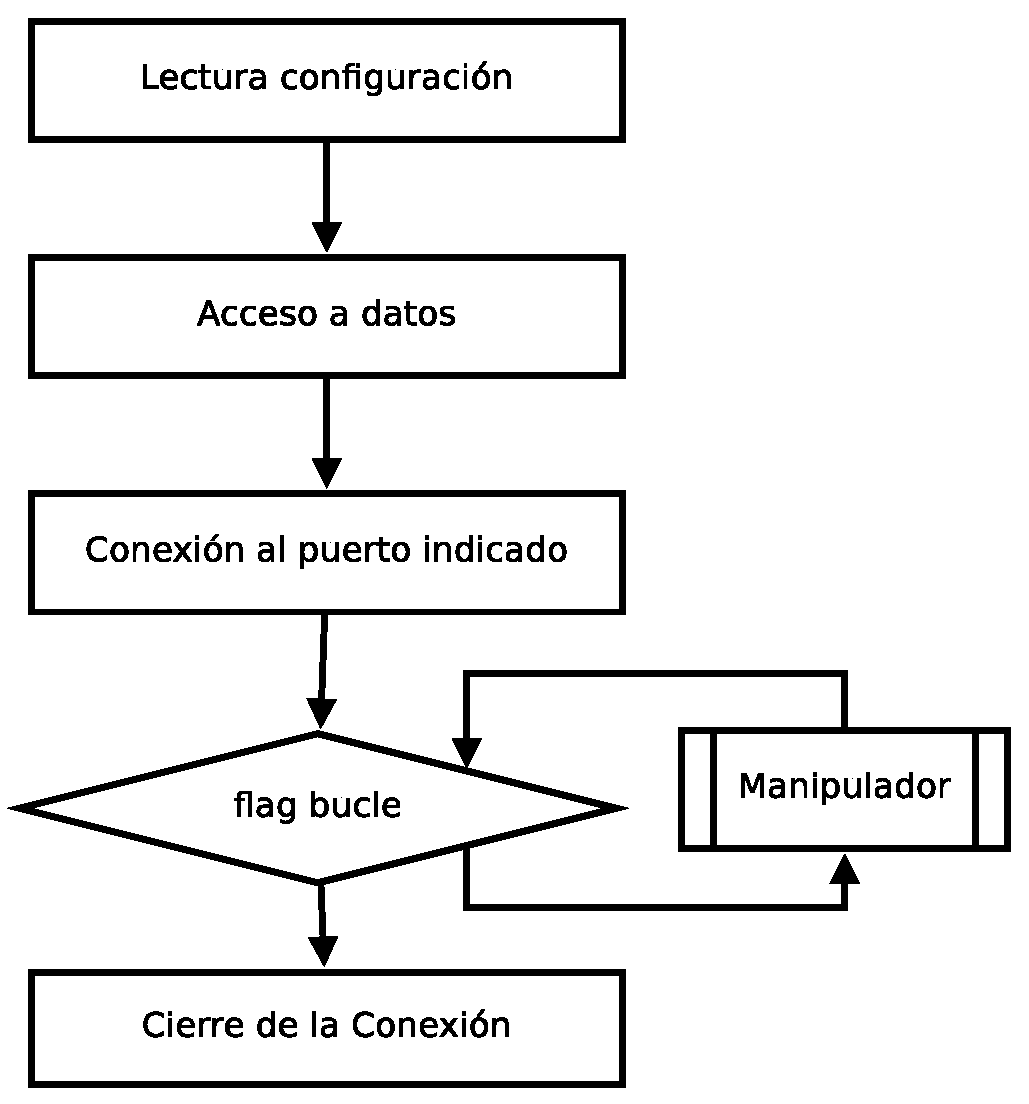
\includegraphics[width=0.45\textwidth]{img/FlujoServicio.eps}
              \caption{Niveles OSI}
  \label{fig:nivelesOSI}
\end{wrapfigure}

Sin embargo la implantación de sistemas de red por capas, enlaces no dedicados y sobre todo la diversificación de equipos mucho mas baratos y potentes han modificado el panorama de manera importante: Además de diversificarse los tipos de servicios era posible que varios de ellos coexisitieran en el mismo equipo.

En el contexto de los sistemas informáticos un protocolo es un conjunto de reglas predefinidas, cuyo proposito es estandarizar actividades y procesos. Siguiendo un mismo protocolo se garantiza que se mantendrá la compatibilidad entre los sistemas involucrados, independientemente del medio sobre el que est\'en en contacto, posiblemente otros protocolos.

La forma cl\'asica de programar un servicio consiste en un bucle de escucha que inicia subprocesos para cada conexi\'on entrante y que finaliza cuando esta acaba o se produce un error. Se presentan dos entidades en este caso, la del servicio que incluiria las rutinas para iniciar la escucha y el acceso a los datos y la del manipulador, que atiende la conexion siguiendo las pautas del protocolo.

\subsection{Servicio}

Al arrancar un servicio antes de iniciar el bucle de escucha deben realizarse una serie de procedimientos:
\begin{enumerate}
	\item La lectura de parámetros desde linea de comandos
	\item La lectura de parámetros desde el archivo de configuracion
	\item El registro de actividad en el(los archivo(s) pertinentes
	\item Preparar el acceso a los datos necesarios, ficheros o bases de datos
\end{enumerate}

\subsubsection{Parámetros}
Existen parametros que son comunes practicamente a cualquier servicio por ejemplo:
\begin{enumerate}
	\item Fichero de configuraci\'on.
	\item N\'umero de puerto para la escucha
	\item N\'umero m\'aximo de conexiones simultaneas
	\item Ficheros de registro, eventos, errores, etc
	\item Nivel de locuacidad (verbosity) en los registros.
\end{enumerate}
O parametros particulares para segun que tipos de servicio:
\begin{enumerate}
	\item Acceso al medio de datos
	\item Parametros de configuraci\'on concretos
\end{enumerate}
Debe tenerse en cuenta que los parametros en el fichero de configuracion tienen menor prevalencia que los indicados por linea de comandos, salvo el que especifique precisamente que fichero de configuracion debe leerse.

\subsubsection{Ficheros de configuración}
Debe acordarse una estructura común a todos los ficheros de configuración que se parsearán desde la plataforma pero permitiendo a la vez mantener la genericidad suficiente como para no perder la flexibilidad que haga este sistema util a cualquier implementacion de servicios y que a su vez permita que los usuarios puedan entender el fichero de forma clara y manipularlo facilmente.

Se espefican con ese fin las siguiente sintaxis:


\[<nombre parametro>=<valor>\{,<valor-N>\}\]


Para los valores que deben utilizar los parametros se pueden utilizar comodines para ampliar la versatilidad:
\begin{enumerate}
	\item \%H - Hostname
	\item \%i - Ip de la conexion entrante
	\item \%p - Puerto de origen de la conexion
	\item \%d - fecha actual
	\item \%t - hora actual
\end{enumerate}

\subsubsection{Locuacidad}
Para que puedan establecerse mensajes de depuración a distintos niveles debe adoptarse un sistema de categorias de mensajes, en cada etapa o proceso del servicio y del manipulador se emiten mensajes que incorporan el nivel de locuacidad para el que son generados, será la clase encargada de mostrar mensajes la que los muestre segun si el nivel de estos es menor o no que el indicado.
Se proponen los siguientes niveles
\begin{enumerate}
	\item 0 - Básico: mensajes de operaciones minimo, inicio del sistema, errores en los procedimientos.
	\item 1 - Moderado: mensajes comunes, entrada en servicio de un manipulador y puntos clave del desarrollo de la atención.
	\item 2 - Productivo: indica la entrada en la mayoria de las etapas de un servicio. Se amplian los detalles de los mensajes de error
	\item 3 - Expresivo: indica la entrada a cada etapa del servicio, se detalla el contexto de cada mensaje de error.
	\item 4 - Locuaz: detalla el contexto de cada etapa.
\end{enumerate}

\subsubsection{Registro}
Con la intencion de simplificar la tarea de gestionar la salida de mensajes, bien a la salida de la consola o a ficheros de registro deben implementarse clases destinadas a tal fin, que vuelquen o no los mensajes al medio según la locuacidad que se ha fijado y que en caso de que el medio predeterminado falle (por falta de espacio o cambio de permisos) sea capaz de cambiar a otro (indicado en la configuracion o a los medios salida por pantalla dedicados a tal fin).


\begin{figure}[h]
	\includegraphics[width=0.95\textwidth]{img/DiagramaClasesAnalisis.eps}
              \caption{Diagrama de Clases de Análisis}
     \label{fig:DiagramaClasesAnalisis}
\end{figure}


\subsection{Manipulador}
Precisamente es la naturaleza de un protocolo, como un conjunto ordenado de etapas en las que se organiza el flujo de informacion entre los sistemas, la que permite abstraer al programa servidor como un automata sensible al contexto. Cada etapa del manipulador equivale al estado del automata y pueden realizarse un conjunto determinado de acciones:
\begin{enumerate}
	\item Recibir datos desde la conexión
	\item Emitir datos a la conexión
	\item Tratar, almacenar o recuperar datos
	\item Avanzar, saltar o retroceder a otra etapa
\end{enumerate}

La recepción de los datos puede además controlarse mediante expresiones regulares según las especificaciones del protocolo, detectando rapidamente errores en la entrada. Debe facilitarse además la adopción de distintos tipos de intercambio de datos, controlados, formato en bruto o encriptados para evitar reimplementaciones de esta clase de rutinas.

En el diseño del manipulador debe tenerse en cuenta que normalmente existe un orden convencional en las etapas, previsiblemente estas deberia contener un numero limitado de procedimientos, para reducir la complejidad.

Durante la implementación de los protocolos ha aparecido la necesidad de trabajar sobre UDP. Para permitir esta funcionalidad y mantener un diseño eficiente se ha optado por dividir el manipulador en tres nuevas clases que permitieran trabajar tanto sobre el protocolo TCP como UDP y en concordancia a sus características:
\begin{enumerate}
	\item{Handler: la clase Handler primitiva se centra en la gestion de estados, el transito entre estos, y su inicializacion.}
	\item{TCPHandler: esta clase que hereda de Handler contiene una version especial de las rutinas de emision y recepcion de datos, se inicializa pasando el hash del socket.}
	\item{UDPHandler: Cada vez que un datagrama llega al servidor se instancia al manipulador, integrando la direccion de origen del datagrama y los datos que portaba, esta clase tendra sus propias rutinas de emisión y recepción. Debe tenerse en cuenta que en este tipo de manipulador se hace necesario algun sistema que permita recuperar desde el servidor en que estado se encontraba al finalizar la última transmision.}
\end{enumerate}
\subsection{Flujos de los protocolos}
A continuación se va a espeficicar el flujo de los protocolos con los que se va a probar la plataforma.

\subsubsection{Telnet}
\begin{figure}[h]
	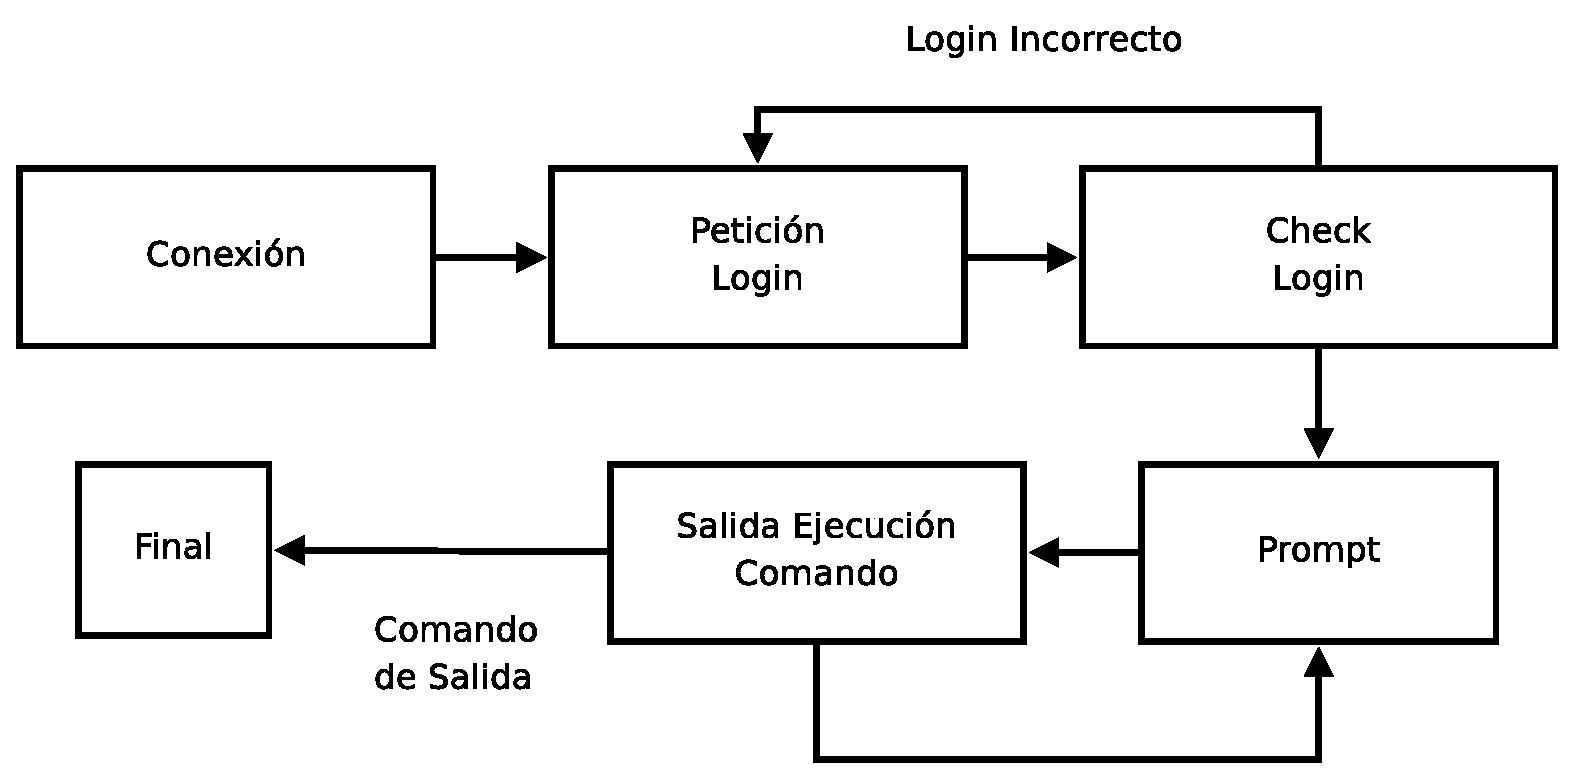
\includegraphics[width=0.95\textwidth]{img/DiagramaFlujoTelnet.eps}
              \caption{Flujo de desarrollo del protocolo Telnet}
  \label{fig:DiagramaFlujoTelnet}
\end{figure}

El protocolo Telnet tiene un flujo básico de desarrollo muy simple:
\begin{enumerate}
	\item Se establece la conexión con el cliente
	\item Se presenta el dialogo de peticion de contraseña y se espera a que se introduzcan los datos.
	\item Se checkea la contraseña contra la base de datos correspondiente
	\item Se solicita el comando a ejecutar en el sistema
	\item Se ejecuta el comando pertinente y se muestra su salida. y se vuelve al paso 4.
\end{enumerate}
Existe un pequeño conjunto de pasos alternativos:
\begin{enumerate}
	\item (4.Alternativo) El usuario debe repetir la autentificación
	\item (5.Alternativo) Se ha solicitado finalizar la sesión con lo que procedemos a la desconexión.
\end{enumerate}
\subsubsection{HyperText Transfer Protocol}
\begin{figure}[h]
	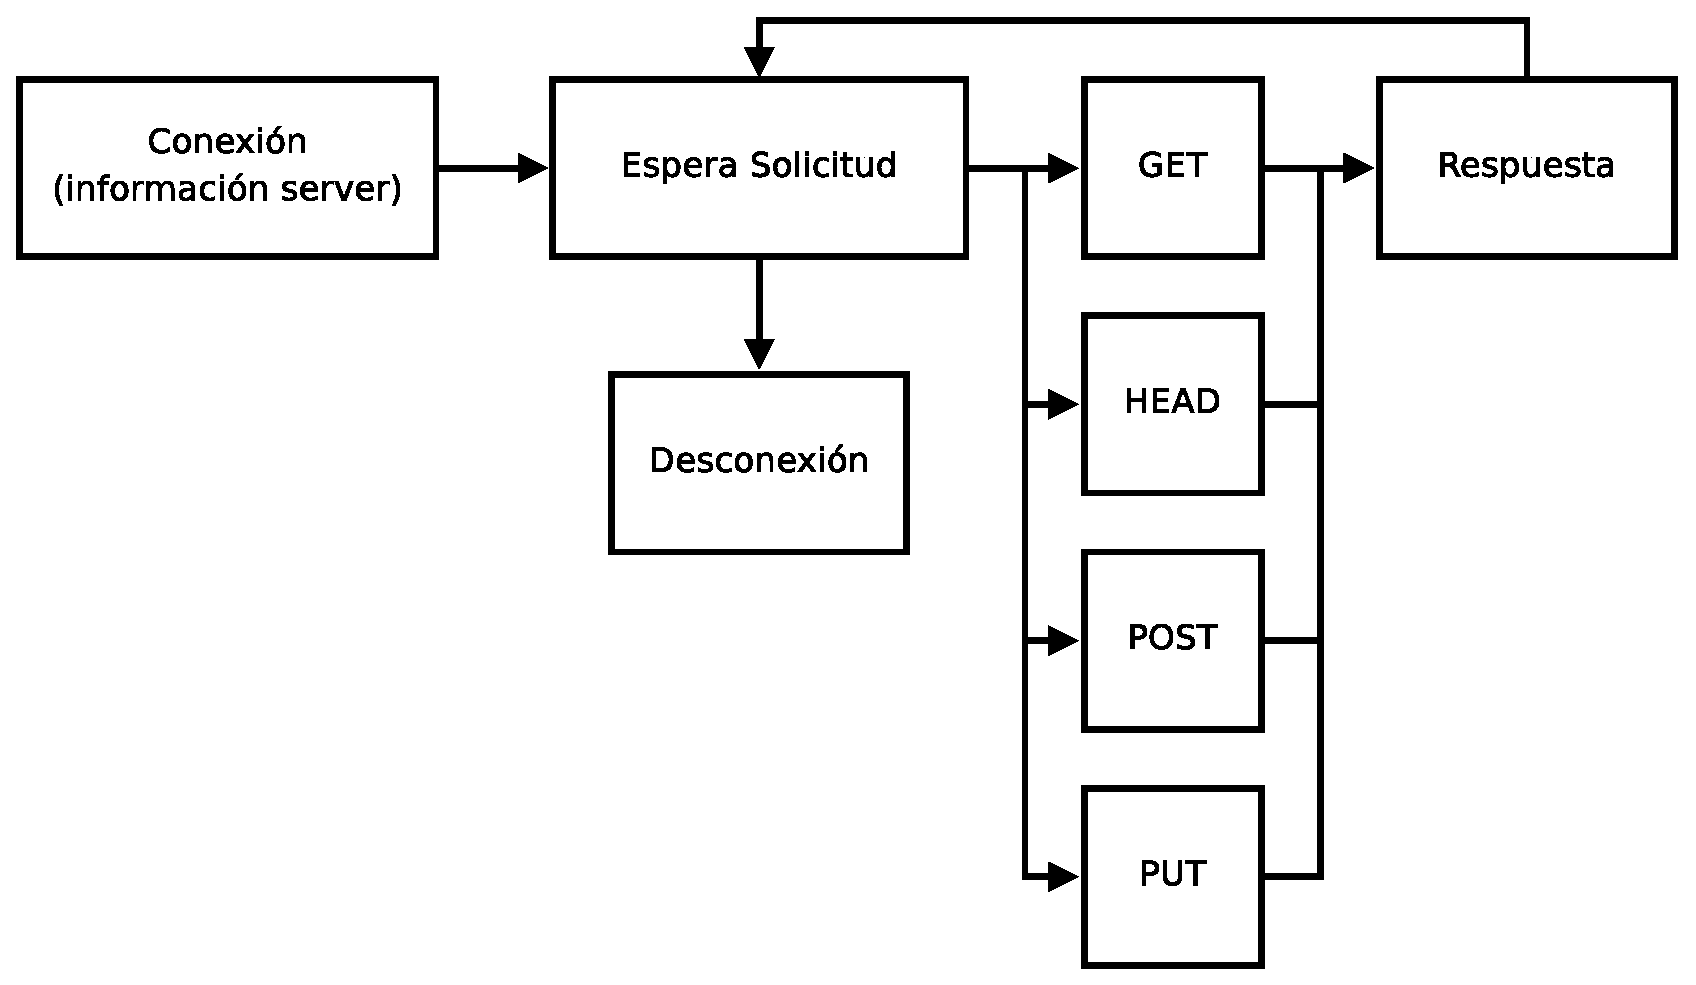
\includegraphics[width=0.95\textwidth]{img/DiagramaFlujoHTTP.eps}
              \caption{Flujo de desarrollo del protocolo HTTP}
  \label{fig:DiagramaFlujoHTTP}
\end{figure}
El protocolo HTTP/1.1 tiene un flujo basico bastante más amplio, ya que despues de recibir la orden las rutinas que atenderán el comando difieren drasticamente, en consecuencia deberán implementarse nuevos estados para cada tipo de comando.
\begin{enumerate}
	\item Se establece la conexión con el cliente
	\item Se muestra la información del servidor
	\item Se reciben las cabeceras y el comando
	\item En el estado de atencion se recibe el resto de la información (si procede)
	\item Se responde informando del estado.
\end{enumerate}
Aunque la conexión pueda perderse inesperadamente en cualquier momento, es en el momento de esperar el comando cuando se produciría una desconexión correcta.
\subsubsection{Session Initialization Protocol}
El protocolo SIP es responsable de varias tareas, aunque puede operar sobre UDP la implementación sobre BLAS solo funcionará sobre UDP. Estas tareas son:
Es precisamente en este punto por la necesidad de trabajar sobre UDP cuando se ha tomado la decisión de dividir el manipulador en tres nuevas clases que permitieran trabajar tanto sobre el protocolo TCP como UDP y en concordancia a sus características.
\begin{figure}[h]
	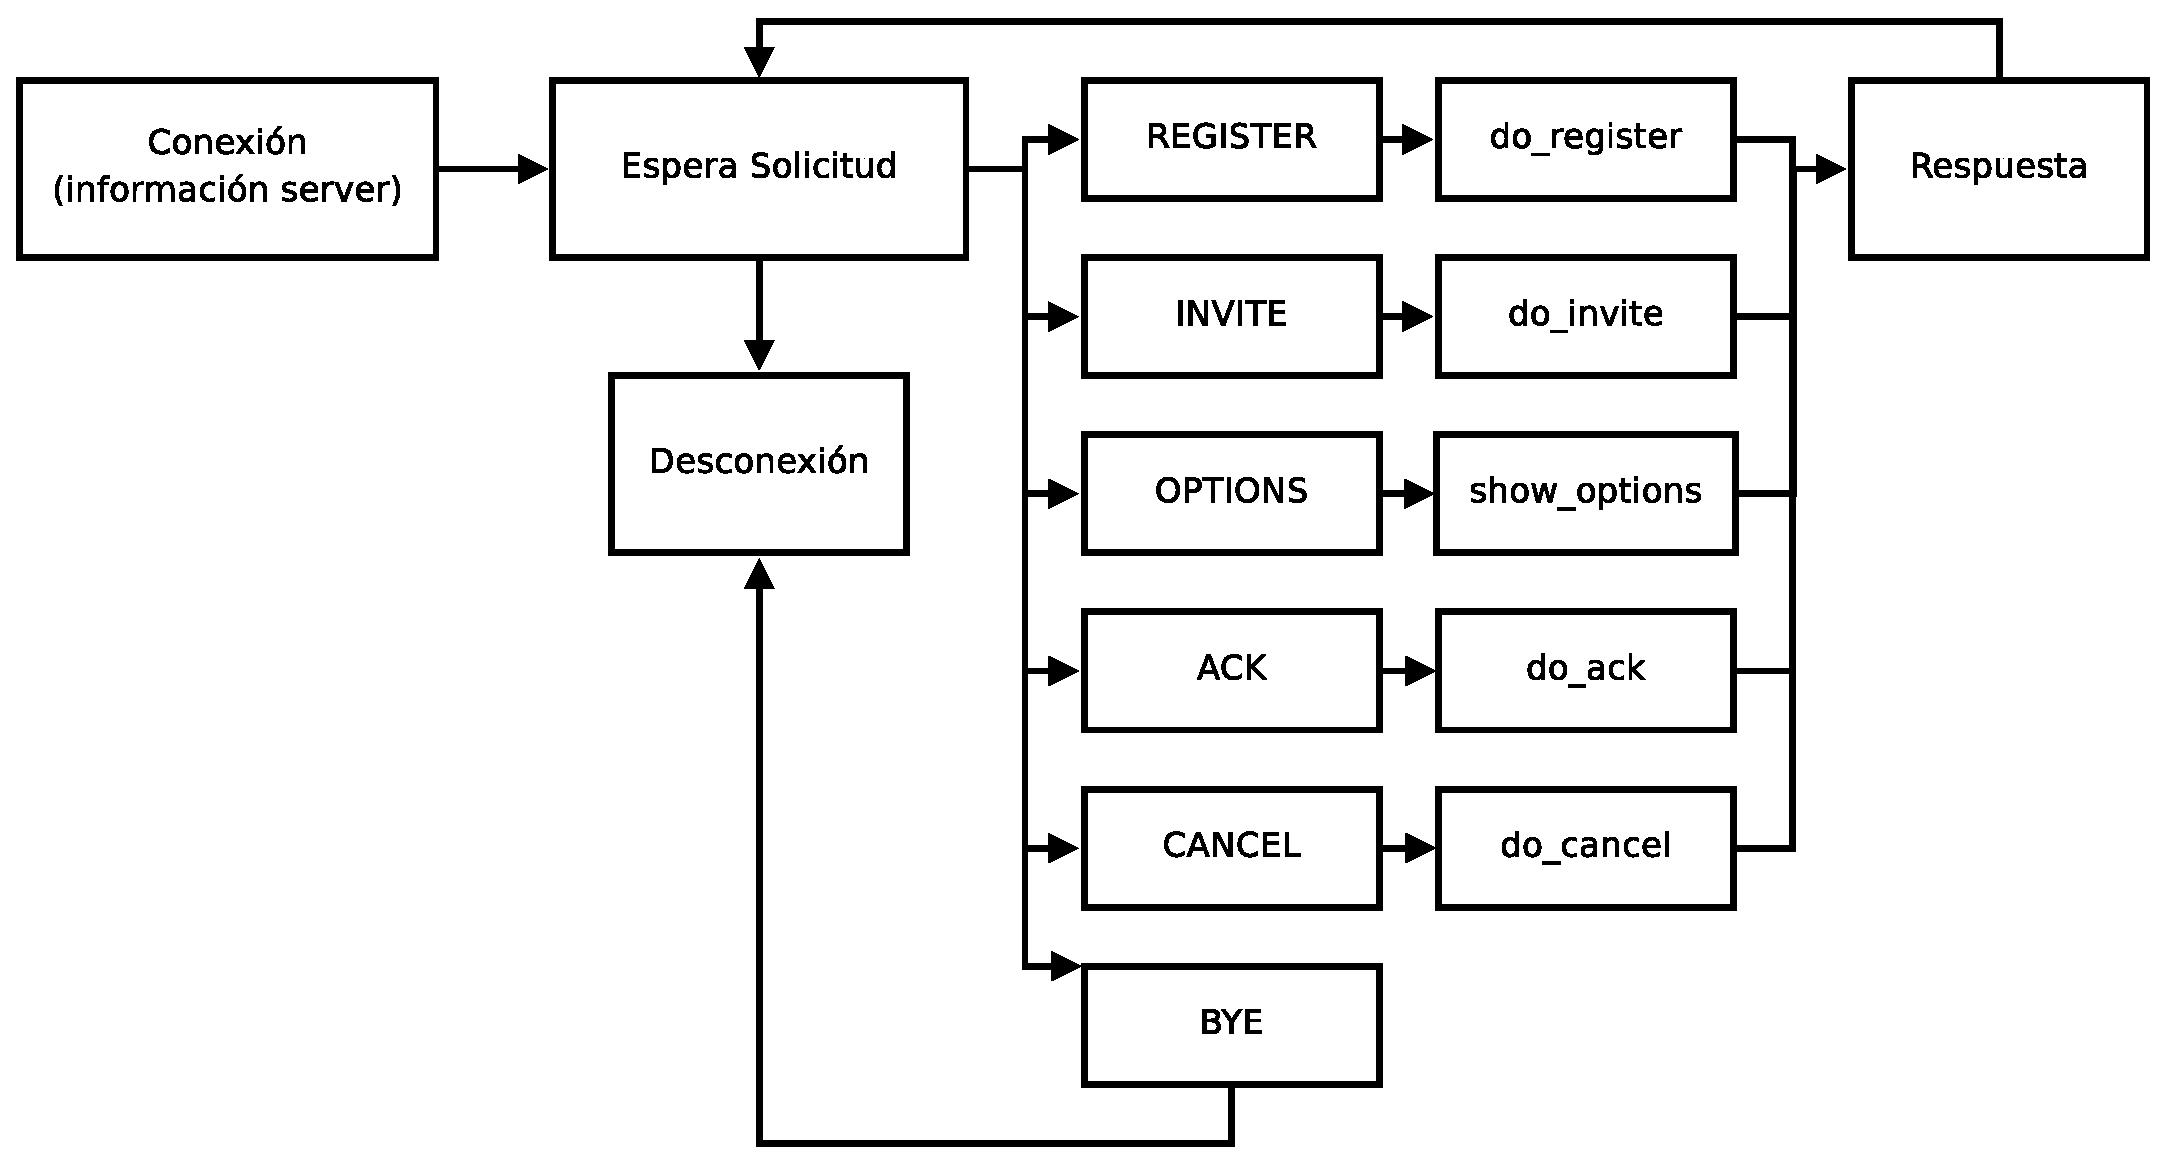
\includegraphics[width=0.95\textwidth]{img/DiagramaFlujoSIP.eps}
              \caption{Flujo de desarrollo del protocolo SIP}
  \label{fig:DiagramaFlujoSIP}

\end{figure}

\begin{enumerate}
	\item{Registro(REGISTER): El usuario se da de alta en el sistema y figura en el directorio de usuario.}
	\item{Invitación(INVITE): Dirigido a un usuario se le autoriza a acceder a un medio compartido. Debe aceptarse con ACK o denegarse con CANCEL.}
	\item{Opciones(OPTIONS): Solicita al servidor el listado de las funcionalidades.}
	\item{Cierre(BYE): Avisa de que va a procederse con la desconexión.}
\end{enumerate}


\subsection{Acceso a datos}
Muchos servicios tienen la necesidad de leer y escribir en medios de datos centralizados, por eso es importante diseñar según se debe hacer un esfuerzo en desarrollar un modelo de acceso a datos que permita una lectura lo más transparente posible, facilitando la lectura del codigo. 

Normalmente existen unos tipos limitados de medios de datos:
\begin{enumerate}
	\item{Registos unificados volátiles: Son medios de datos que se borrarán cuando se desactive el servicio, deben permitir el acceso concurrente por parte de los hilos. Este tipo de medios sería muy adecuado para sistemas de chat etc.}
	\item{Accesos a bases de datos: Python tiene soporte para acceder a muchos tipos de bases de datos: Mysql, Postgresql, ODBC, etc. Sin embargo diseñar un acceso a datos mediante objetos que eviten la manipulacion de peticiones SQL en el codigo de la atención del servicio será básico para la comprensión del codigo y su depuración}
	\item{Acceso remoto a datos: En ocasiones los datos que se necesitan estarán en sistemas remotos, accediendo a ellos mediante conexiones IP/TCP y normalmente sobre estos metodos HTTP, SOAP o REST. Al igual que en otros medios de acceso es importante que el metodo de acceso se abstraiga del codigo de atención del servicio}
\end{enumerate}
En definitiva y aunque para cada tipo de servicio el modelo de acceso a datos varía considerablemente se pueden establecer las siguientes lineas para el analisis y la orientación que tomará el sistema:
\begin{enumerate}
	\item{Claridad: Debe evitarse la molesta aparición de lineas SQL, peticiones HTTP, XML y similares en el codigo.}
	\item{Orientación a objetos: Un buen modelo de acceso a datos reducirá sensiblemente el tiempo que se requiera para depuración y posteriores.}
	\item{Manejo de errores: Es importante integrar el manejo de excepciones en las rutinas de adquisición de datos ya que no estarán exentas de fallos.}
	\item{Oportunidad de acceso: Deben elegirse adecuadamente en que momentos se accederá a los datos, para no producir latencias en puntos del proceso sensibles al tiempo de respuesto.}
\end{enumerate}

\section{Diseño}

\subsection{Librería principal}
Existe una parte común a toda la plataforma que contiene las clases abstractas, puede verse su diagrama de clases de diseño en la figura \ref{fig:DiagramaClasesDiseñoCore}

\begin{figure}[h]
	\includegraphics[width=0.80\textwidth]{img/DiagramaClasesDisennoCore.eps}
	\caption{Diagrama de Clases de la librería principal} 
	      \label{fig:DiagramaClasesDiseñoCore}
\end{figure}

En estas clases se incorporarán todas las funcionalidades que puedan emplearse desde cualquier implementación de un servicio. Para simplificar el procedimiento de herencia de componentes se incluiran todas en el archivo core.py, que acompañaría al archivo que contenga el código del servicio en si mismo en cada despliegue que se haga a posteriori del sistema.
\subsubsection{Server}
Esta clase incluye las rutinas necesarias para la inicializacion y configuración del servicio:
\begin{enumerate}
	\item Carga y parseado de los parámetros de linea de comando.
	\item Carga e interpresatcion de los archivos de configuración.
	\item Reserva del socket al que se conectarán los clientes del servicio.
	\item Bucle principal de inicializacion y despacho de los hilos.	
	\item Inicialización de los registros de eventos y errores del sistema.
	\item Recopilación de las cadenas de documentación relacionadas con cada parametro del sistema.
	\item Inicialización de los medios de acceso a datos comunes (si procede). 
\end{enumerate}
\subsubsection{Error}
Esta clase que hereda de la clase de sistema Exception se utiliza como tipo de datos por defecto en caso de que alguno de los procesos o rutinas del sistema no pueda realizar su función, en estos casos devolverá un objeto de clase Error.

Además Error contiene 2 datos importantes para la infraestructura:
\begin{description}
	\item[msg]Cadena que contiene una cadena explicando el suceso que originó el error.
	\item[level]Entero que se utiliza para saber si la gravedad del suceso obliga a su aparición en los registros.
\end{description}
Los metodos son una sobrecarga de los metodos basicos de la clase Exception:
\begin{description}
	\item[\_\_init\_\_]Que inicializa el objeto proveyendo de la información con el mensaje de error y el nivel de importancia.
	\item[\_\_str\_\_]Devolverá la cadena con la explicación del error y el nivel de importancia cuando se necesite imprimirlo en el registro.
\end{description}
\subsubsection{Log}
En esta versión del registro solo se volcarán los eventos y errores a salida estandar o a ficheros. Para reducir el acoplamiento en las llamadas en los objetos de registro integran los siguientes datos durante su tiempo de vida:
\begin{description}
	\item[file]File salvo que su valor sea None será el descriptor de fichero donde se volcará la información.
	\item[level]Int indicará el nivel de importacia que debe igualarse o superarse para que el evento se vuelque en el registro.
\end{description}
Los m\'etodos propios de los objetos tipo Log son:
\begin{description}
	\item[\_\_init\_\_()]M\'etodo de inicialización del registro, indicando el nombre del fichero de volcado y el nivel mínimo de importancia. Si la apertura del fichero falla se pasarán a volcar los datos a la salida estandar.
	\item[put()]Con este m\'etodo se vuelcan eventos al registro, además del mensaje debe acompañarse del nivel de importancia del evento. Para simplificar su invocación normalmente se utiliza un puntero desde self.log[``report''].put() a self.report() con lo que las llamadas son mucho más cortas.
\end{description}
\subsubsection{Handler: UDP y TCP}
Seguramente las clases más importantes que se incorporan en un servicio:
\begin{enumerate}
	\item Handler: Es la clase principal, hereda de la clase hilo (Thread) y sus principales funcionalidades son:
		\begin{enumerate}
			\item Controlar el avance, retroceso y transito entre estados del manipulador en ejecución.
			\item Sobrecargar las clases minimas de la clase Thread para un funcionamiento coherente.
		\end{enumerate}
	\item TCPHandler: Versión del manipulador que contiene los atributos y m\'etodos concretos para tratar con el socket que les corresponda, en este caso basta con guardar el puntero al Socket, ya que es lo unico que necesitan las rutinas send() y receive() para enviar y recibir datos con el cliente.
	\item UDPHandler: Versión del manipulador destinada a atender las peticiones UDP. En el caso de protocolo UDP es más complicado ya que no existe un Socket como tal, en su lugar se guardar la ip y puerto de donde procedía la comucación y ademas el buffer de los datos recibidos. Con lo que los procedmientos de envio y recepción de datos tienen las siguientes particularidades:
		\begin{enumerate}
			\item send(): debe crear un nuevo socket UDP con los datos de conexión que posee, estos pueden facilitarse desde los parámetros o utilizar los que figuran como origen de los datos. No existe confirmación sobre si los datos han llegado por lo que la aplicación debe buscar su forma de confirmar la transmisión.
			\item receive(): Todos los datos que puedan llegar al hilo de atención llegan de una sola vez desde el momento en que se inicia, se van consumiendo según especifique el patrón que se pasa como parámetro. Si el buffer de datos está vacio se devolvera un Error.
		\end{enumerate}
\end{enumerate}
\subsection{Servicio de ejemplo}
A continuación se presenta un ejemplo de como se realiza la implementación de un servicio heredando de las clases de BLAS. En la figura \ref{fig:DiagramaClasesDiseñoParticular} puede observarse como se relacionan las clases.

\begin{figure}[h]
	\includegraphics[width=0.80\textwidth]{img/DiagramaClasesDisennoParticular.eps}
	\caption{Diagrama de Clases de un servicio de ejemplo} 
	      \label{fig:DiagramaClasesDiseñoParticular}
\end{figure}
El arranque del sistema se realiza de la siguiente manera:
\begin{enumerate}
	\item Se carga el fichero con el interprete de python, presumiblemente el fichero se llamaría particular.py.
	\item Una vez finalizadas las importaciones de los modulos se cargan las definiciones de clases y sus m\'etodos.
	\item Cuando se llega a la zona de ejecución se instancia un objeto ParticularServer con los argumentos recibidos por linea de comandos, despu\'es se invoca al m\'etodo mainloop indicandole la clase de manipulador que debe instanciar.
	\item Durante la inicializacion de un objeto ParticularServer se instancian a su vez los objetos de registro, a su vez se llama a la inicializacion de Server, que será común a todos los servidores, aqui se parsearán las opciones de la linea de comandos, cuyas directrices estarán distribuidas en el codigo de ParticularServer y Server en m\'etodos que inician su nombre con ``config\_'' seguido del nombre del parámetro, en su campo de documentación se incluye el prefijo que debe utilizarse en la linea de comandos para modificar estos parámetros.
	\item En mainloop() discriminando el tipo de manipulador(TCP o UDP) abrirá el tipo de socket pertinente e iniciará un bucle while. Dentro de estelas conexiones se irán atendiendo por parte de los manipuladores. Para que los manipuladores puedan hacer su trabajo deben primero inicializarse y luego emitir la orden de arranque.
	\item Al inicializar el hilo del manipulador se le aporta bien el socket de conexión para los tipo TCP y el buffer y la dirección de origen para los UDP. El m\'etodo start() que se hereda de la clase Thread iniciará la ejecución del hilo que se desarrollará a lo largo de los estados que se deban seguir para atender la petición.
	\item la mayor parte del codigo del manipulador serán m\'etodos cuyo nombre empiece port ``step\_'' seguido del identificador del paso en si mismo, en cada paso debe indicarse si se pasa al siguiente, al anterior o se salta a otro, de otra manera se repetirá el mismo paso.
\end{enumerate}
\subsection{Servicio Telnet}
Para imitar un servicio de terminal interactiva con autentificación 
			  \ref{fig:DiagramaClasesDisennoTelnet}
\begin{figure}[h!]
		\begin{center}
				\includegraphics[angle=90,width=0.90\textwidth]{img/DiagramaClasesDisennoTelnet.eps}	
			\end{center}
			\caption{Diagrama de Clases de Diseño: Servicio Telnet}
			  \label{fig:DiagramaClasesDisennoTelnet}
\end{figure}

\subsection{Servicio HTTP}

\begin{figure}[h!]
		\begin{center}
				\includegraphics[angle=90,width=0.90\textwidth]{img/DiagramaClasesDisennoHTTP.eps}	
			\end{center}
			\caption{Diagrama de Clases de Diseño: Servicio HTTP}
			  \label{fig:DiagramaClasesDisennoHTTP}
\end{figure}

\subsubsection{Bifurcación y flujo de estados} 
Una vez que el servidor ha recibido la trama con la petición e instanciado el hilo de atención correspondiente se inicia el siguiente proceso:
\begin{description}
	\item[Request] En este paso se recibe la primera linea de la petición, se informa en el registro del origen de la transmisión y se almacena el comando en los datos del hilo. Se pasa a la etapa Run.
	\item[Headers] Este paso irá recolectando y parseando las cabeceras de las peticiones, no se pasará al siguiente paso Run hasta que se encuentre con una cabecera en blanco.
	\item[Run] La funcion de este estado es elegir a cual se pasará según el comando que se ha recibido.
	\begin{description}
		\item[Run\_Get] En este paso se relativizará la ruta solicitada a la que esta configurada como raiz del servidor, además si no se ha indicado un fichero se intentará localizar ``index.html''. Si al intentar la apertura del fichero se produce una excepción será capturada y se emitirá al cliente una respuesta ``404 Not Found''. En caso de que la apertura del fichero sea correcta se emitirá antes un mensaje ``200 OK'', las cabeceras de información mínimas, incluyendo el tamaño del contenido a transmitir y finalmente el cuerpo de la petición. A continuación se indicará que el estado siguiente es ``End''.
	\end{description}
	\item[End] Esta parte del proceso guardará la información obtenida de los pasos anteriores y emitirá el suceso del fin de la petición al registro de eventos.
\end{description}
Puede encontrarse el diagrama de clases de diseño en \ref{fig:DiagramaClasesDisennoHTTP} 
\subsection{Servicio SIP}
\begin{figure}[h]
		\begin{center}
				\includegraphics[angle=90,width=0.90\textwidth]{img/DiagramaClasesDisennoSIP.eps}	
			\end{center}
			\caption{Diagrama de Clases de Diseño: Servicio SIP}
			  \label{fig:DiagramaClasesDisennoSIP}
\end{figure}
\subsubsection{Bifurcación y flujo de estados} 
Una vez que el servidor ha recibido la trama con la petición e instanciado el hilo de atención correspondiente se inicia el siguiente proceso:
\begin{description}
	\item[Request] En este paso se recibe la primera linea de la petición, se informa en el registro del origen de la transmisión y se almacena el comando en los datos del hilo. Se pasa a la etapa Run.
	\item[Headers] Este paso irá recolectando y parseando las cabeceras de las peticiones, no se pasará al siguiente paso Run hasta que se encuentre con una cabecera en blanco.
	\item[Run] La funcion de este estado es elegir a cual se pasará según el comando que se ha recibido.
	\begin{description}
		\item[Run\_Register] Este paso acaba procesando cualquier comando Register, si no hay autentificación la solicita generando antes un codigo ``nonce'' de desafio para que el cliente responda, a continuación emite un ``401 Unauthorized'' con la información del desafio. En caso de que el cliente haya aportado autentificación se llama al metodo ``digest'' para realizar el contraste del campo ``response'' y la respuesta producida por el propio servidor. A continuación se procederá al estado ``End''.
		\item[Run\_Subscribe] En este estado se guarda información de usuario en el registro para aviso de eventos. A continuación se pasa al estado ``End''.
		\item[Run\_Invite] En este estado si tanto el usuario origen como destino estan validados se pasa al estado ``Invite\_Request'', en caso contrario se pasará a ``End''.
		\begin{description}
			\item[Invite\_Request] En este estado se enviará una petición al destinatario para que acepte la solicitud, se pasará al estado ``End'' despues de marcar la invitacion como pendiente.
		\end{description}
		\item[Run\_Ack] Se revisa en el registro de invitaciones pendientes si existe registro con esa referencia, de ser así se enviarán una confirmación al emisor de la misma y se pasará al estado ``End''.
	\end{description}
	\item[End] Esta parte del proceso guardará la información obtenida de los pasos anteriores y emitirá el suceso del fin de la petición al registro de eventos.
\end{description}
\subsubsection{Autentificación}
El procedimiento de autentificación en SIP se realiza a trav\'es de un mecanismo heredado de HTTP Digest. para que se produzca la autentificación se desarrolla la siguiente secuencia:
\begin{enumerate}
	\item El cliente pide registrarse en el servicio. No prove\'e m\'etodo de contraste alguno.
		\scriptsize
		\begin{verbatim}
		REGISTER sip:192.168.1.100 SIP/2.0
		Tue Aug 26 21:09:38 2008:192.168.1.11:5072:current state:receiving param
		CSeq: 127 REGISTER
		Via: SIP/2.0/UDP 192.168.1.11:5072;branch=z9hG4bK2686af38-1072-dd11-9855-0016e6dfa1a5;rport
		User-Agent: Ekiga/2.0.12
		From: <sip:edorka@192.168.1.100>;tag=4279af38-1072-dd11-9855-0016e6dfa1a5
		Call-ID: 205faf38-1072-dd11-9855-0016e6dfa1a5@Newton
		To: <sip:edorka@192.168.1.100>
		Contact: <sip:edorka@192.168.1.11:5072;transport=udp>
		Allow: INVITE,ACK,OPTIONS,BYE,CANCEL,NOTIFY,REFER,MESSAGE
		Expires: 3600
		Content-Length: 0
		Max-Forwards: 70
		\end{verbatim}
		\normalsize
	\item El servidor contesta con un error ``401 Unauthorized`` y provee en las cabeceras del desafio de autentificación.
		\scriptsize
		\begin{verbatim}
		SIP/2.0 401 Unathorized
		WWW-Authenticate: Digest realm=``192.168.1.100'', nonce=``ff8c..'', qop=``auth''
		CSeq: 102 REGISTER
		Via: SIP/2.0/UDP 192.168.1.11:5069;branch=z9hG4bKc2448342-...;rport=5069
		From: <sip:edorka@192.168.1.100>;tag=5c418342-f671-dd11-9855-0016e6dfa1a5
		Call-ID: 00a1a017-e771-dd11-9855-0016e6dfa1a5@Newton
		To: <sip:edorka@192.168.1.100>;tag=5c418342-f671-dd11-9855-0016e6dfa1a5
		Contact: <sip:edorka@192.168.1.11:5069;transport=udp>
		Content-Length: 0
		Server: PythonSIP prototype
		\end{verbatim}
		\normalsize
	\item El cliente reintenta el registro en el servidor incluyendo en la cabecera un campo ''Authorization'' con los datos que ha empleado para calcular el campo ``response''.
		\scriptsize
		\begin{verbatim}
		REGISTER sip:192.168.1.100 SIP/2.0
		CSeq: 129 REGISTER
		Via: SIP/2.0/UDP 192.168.1.11:5072;
			branch=z9hG4bK2870b438-1072-dd11-9855-0016e6dfa1a5;rport
		User-Agent: Ekiga/2.0.12
		Authorization: Digest username=``edorka'', realm=``192.168.1.100'', 
			nonce=``ff8cf8e764fca9134c1cd5499bc4684b'', uri=``sip:192.168.1.100'', 
			algorithm=md5, response=``365cf4061c002b09c75408a4907ac911'', 
			cnonce=``3261b438-1072-dd11-9855-0016e6dfa1a5'', 
			nc=``00000001'', qop=``auth''
		From: <sip:edorka@192.168.1.100>;tag=4279af38-1072-dd11-9855-0016e6dfa1a5
		Call-ID: 205faf38-1072-dd11-9855-0016e6dfa1a5@Newton
		To: <sip:edorka@192.168.1.100>
		Contact: <sip:edorka@192.168.1.11:5072;transport=udp>
		Allow: INVITE,ACK,OPTIONS,BYE,CANCEL,NOTIFY,REFER,MESSAGE
		Expires: 3600
		Content-Length: 0
		Max-Forwards: 70
		\end{verbatim}
		\normalsize
	\item Si el servidor da por buena la respuesta al desafio despu\'es de calcularlo por su cuenta emitirá una respuesta ``200 OK'' en referencia a la última petición.
		\scriptsize
		\begin{verbatim}
		SIP/2.0 200 OK
		CSeq: 107 REGISTER
		Via: SIP/2.0/UDP 192.168.1.11:5069;
			branch=z9hG4bK460a1e59-0572-dd11-9855-0016e6dfa1a5;rport=5069
		From: <sip:edorka@192.168.1.100>;tag=da541c59-0572-dd11-9855-0016e6dfa1a5
		Call-ID: 00a1a017-e771-dd11-9855-0016e6dfa1a5@Newton
		To: <sip:edorka@192.168.1.100>;tag=da541c59-0572-dd11-9855-0016e6dfa1a5
		Contact: <sip:edorka@192.168.1.11:5069;transport=udp>
		Content-Length: 0
		Server: PythonSIP prototype
		\end{verbatim}
		\normalsize
\end{enumerate}
Para calcular el response correcto se ha implementado un m\'etodo digest() al que se pueden pasar como argumentos el metodo que lo ha llamado y la contraseña que se debe comprobar, el proceso de ``digestión'' es el siguiente
\begin{enumerate}
	\item \begin{math} S1 = MD5(<username>:<realm>:<password>) \end{math}
	\item \begin{math} S2 = MD5(<metodo>:<URI>:) \end{math}
	\item \begin{math} RESP = MD5(S1:<nonce>:<nc>:<cnonce>:<qop>:S2) \end{math}
\end{enumerate}
\section{Manual de usuario}
Para ejecutar cualquiera de los servicios debe situarse en la raiz del CD que acompaña a la memoria y ejecutar el interprete de python indicando el fichero del servicio, por ejemplo:
\begin{verbatim}
python telnet.py
python http.py
python sip.py
\end{verbatim}.

Debe tenerse en cuenta de que para pueda escribirse en el medio los registros de eventos y errores deben copiarse al disco duro los ficheros contenidos en el CD y ejecutar desde ahí. 

El interprete incluido en el CD puede funcionar sin instalación, sin embargo se ha incluido una copia del instalador para windows de la ultima versión disponible de python.

Al ser multiplataforma el interprete y con el, \'el entorno, sabiendo que las reglas y permisos de cada sistema serán diferentes y para evitar problemas en la ejecución se han modificado los puertos de escucha, con lo que telnet estará a la escucha en el puerto TCP 2300 y el servidor HTTP en el puerto TCP 8000. El protocolo SIP estará a la escucha en su puerto habitual, 5060 UDP.


\chapter{Conclusiones, previsiones y proyectos futuros}
\section{Conclusiones}
A lo largo de la realización del proyecto se han presentado varias dificultades, que se detallan a continuacion:
\begin{enumerate}
	\item Problemas en la depuración de expresiones regulares, para corregir un fallo durante la entrada de datos aunque este se hubiera localizado en la expresión regular su corrección resultaba bastante engorrosa. El proceso para comprobarla consistia en abrir un interprete python a parte importar los modulos correspondientes e imitar el mismo procedimiento que realiza el programa, lo que supone escribir 10 lineas de código que irremediablemente se perderán, para evitar esto sería interesante escribir alguna clase de utilidad.
	\item Problemas con los clientes, ya que muchos de estos no se acomodan correctamente a las especificaciones del protocolo, salvo en los casos en que se ha podido llegar a una solución elegante, realizando pequeñas variaciones, aceptar modificicaciones sobre los protocolos normalmente ha implicado producir bastante código extra para subsanarlo.
	\item Las especificaciones RFC son en muchos casos dificiles de entender, para la implementación de los protoclos se ha hecho necesaria capturasde operaciones de dichos protocolos para comprender realmente lo que ocurre.
	\item Aun a pesar de utilizar un importante número de trazas a lo largo del la programación del servicio muchos errores solo pueden localizarse analizando el trafico, por ello disponer de programas como wireshark \url{http://www.wireshark.org/} puede resultar de gran utilidad.
\end{enumerate}
Sin embargo en este proyecto si se han superado obstaculos en un tiempo menor de los esperado:
\begin{enumerate}
	\item El soporte para Datagram User Protocol se implementó en apenas 3 horas, las diferencias con la versión que manejaba sockets TCP eran menores de lo esperado y la facilidad de implementación en python redujo de manera importante el tiempo de implementación.
	\item Los módulos que incorpora Python para casi cualquier necesidad imaginable reduce el tiempo de implementación, sin embargo debe tenerse en cuenta de que estos modulos deben estar presentes tambi\'en en los entornos donde vaya a ejecutarse el servicio.
	\item Las estructuras de datos primitivas de python como listas y diccionarios han resultado muy utiles a la hora de almacenar la información de las cabeceras, al igual que las rutinas para tratamiento de cadenas.
	\item 
\end{enumerate}
El diagrama de diseño de clases del servicio SIP esta en la figura \ref{fig:DiagramaClasesDisennoSIP}

\section{Mejoras}

En futuras implementaciones de BLAS se preveen una serie de mejoras planteadas para aumentar la funcionalidad de la plataforma o solventar sus carencias

\subsection{Cifrado}
Actualmente casi todos los servicios de red se comunican empleando canales seguros. Probablemente imitar cualquier servicio de forma completa requeriría aportar el soporte de distintos metodos criptograficos. Algunos de los algoritmos mas comunes que se pueden localizar en internet son:
\begin{enumerate}
	\item{DES y 3DES: Publicados en 1976 y 1978 respectivamente son los algoritmos más veteranos y aun presentes en muchos sistemas aunque hayan perdido robusted con el paso del tiempo.}
	\item{IDEA: Publicado en 1991 para sustituir a DES}
	\item{Blowfish: Publicado en 1993}
	\item{RC5: Publicado por RSA en 1994}
\end{enumerate}
Para facilitar su uso por parte del programador y así mantener uno de los principales valores de la plataforma deben diseñarse metodos para que una vez negociada una contraseña común el flujo de datos pueda mantenerse de forma identica al uso que se realizara sobre send() y receive(). Ya que python permite la sobrecarga de metodos desde la propia clase durante la ejecución implementar una rutina que reemplace los metodos de entrada y salida no revestirá dificultad.

\subsection{Sistemas de registro opcionales}
Además del volcado de la información de registros de operación y errores al sistema de ficheros o a la salida estandar, existen otras posibilidades que pueden extender la funcionalidad de la plataforma:
\begin{figure}[h] %{h}{0.65\textwidth}
	%{figure}[h]
	\includegraphics[width=0.65\textwidth]{img/DiagramaClasesDisennoNewLogs.eps}	
              \caption{Diagrama de diseño nuevos registros}
  \label{fig:DiagramaClasesDisennoNewLog}
\end{figure}

\begin{enumerate}
	\item{Terminal TCP: Consistente en un servicio que tras conectarse mediante telnet permita revisar los eventos en el sistema.}
	\item{Volcado UDP: se enviarán a una ip y puerto predeterminados la información en texto claro de los eventos del sistema.}
\end{enumerate}

De esta manera se debería extender la clase Log, creando nuevas subclases que heredarian de Log, sobrecargando los metodos para actuar de forma transparente al programador.


\subsection{Establecimiento como servicio del sistema}
Ya que python es multiplataforma según BLAS madure deberían acompañarsele procedimientos faciles para que los servicios producidos puedan implantarse en el sistema junto a otros.

Es importante implementar una rutina que permita un empaquetado facil del codigo y el software asociado (el imterprete Python con el juego de librerias necesario) para un despliegue del sistema lo mas agil y rápido posible.

\subsection{Construcción de expresiones regulares}
La construcción de expresiones regulares que acepten cadenas de acuerdo a un patron consumen tiempo y en ocasiones son el origen de fallos dificiles de diagnosticar. Por este motivo implementar un sistema para construir expresiones regulares de forma rapida y clara debería ser una de las prioridades a la hora de extender el proyecto.

El resultado ideal sería conseguir que no aparezcan expresiones regulares que entorpezcan la lectura del codigo de atención del servicio.
\section{Rendimiento y pruebas}
Para profundizar en las capacidades de la plataforma para implementar servicios en cierto nivel de producción deberían realizarse una serie de estudios
\subsection{Benchmarking}
Comparando con el rendimiento de otros servicios implementados sobre lenguajes mas ligeros como C debería ofrecer una idea de que necesidad de recursos tiene la plataforma en funcion de la cantidad de clientes y el tipo de exigencia de estos. Conociendo estos requisitos podrán conocerse las posibilidades reales de que el prototipo pueda entrar en algún nivel de producción.

Sería interesante realizar distintos intentos según el nivel de optimización con que se configure la compilación a bytecode del producto.


\subsection{Seguridad}
Para obtener datos fiables sobre la confiabilidad del servicio producido, sobretodo si está expuesto a accesos de terceros, deben realizarse pruebas con intención de desestabilizar el programa o incluso acceder a recursos restringidos a traves de el.


\chapter{Anexo}
\section{Licencia GNU Free Documentation License}
 \begin{center}

       Version 1.2, November 2002


 Copyright \copyright{} 2000,2001,2002  Free Software Foundation, Inc.
 
 \bigskip
 
     51 Franklin St, Fifth Floor, Boston, MA  02110-1301  USA
  
 \bigskip
 
 Everyone is permitted to copy and distribute verbatim copies
 of this license document, but changing it is not allowed.
\end{center}

\section{Preamble}

The purpose of this License is to make a manual, textbook, or other
functional and useful document ``free'' in the sense of freedom: to
assure everyone the effective freedom to copy and redistribute it,
with or without modifying it, either commercially or noncommercially.
Secondarily, this License preserves for the author and publisher a way
to get credit for their work, while not being considered responsible
for modifications made by others.

This License is a kind of ``copyleft'', which means that derivative
works of the document must themselves be free in the same sense.  It
complements the GNU General Public License, which is a copyleft
license designed for free software.

We have designed this License in order to use it for manuals for free
software, because free software needs free documentation: a free
program should come with manuals providing the same freedoms that the
software does.  But this License is not limited to software manuals;
it can be used for any textual work, regardless of subject matter or
whether it is published as a printed book.  We recommend this License
principally for works whose purpose is instruction or reference.

\section{Applicability and definitions}

This License applies to any manual or other work, in any medium, that
contains a notice placed by the copyright holder saying it can be
distributed under the terms of this License.  Such a notice grants a
world-wide, royalty-free license, unlimited in duration, to use that
work under the conditions stated herein.  The ``\textbf{Document}'', below,
refers to any such manual or work.  Any member of the public is a
licensee, and is addressed as ``\textbf{you}''.  You accept the license if you
copy, modify or distribute the work in a way requiring permission
under copyright law.

A ``\textbf{Modified Version}'' of the Document means any work containing the
Document or a portion of it, either copied verbatim, or with
modifications and/or translated into another language.

A ``\textbf{Secondary Section}'' is a named appendix or a front-matter section of
the Document that deals exclusively with the relationship of the
publishers or authors of the Document to the Document's overall subject
(or to related matters) and contains nothing that could fall directly
within that overall subject.  (Thus, if the Document is in part a
textbook of mathematics, a Secondary Section may not explain any
mathematics.)  The relationship could be a matter of historical
connection with the subject or with related matters, or of legal,
commercial, philosophical, ethical or political position regarding
them.

The ``\textbf{Invariant Sections}'' are certain Secondary Sections whose titles
are designated, as being those of Invariant Sections, in the notice
that says that the Document is released under this License.  If a
section does not fit the above definition of Secondary then it is not
allowed to be designated as Invariant.  The Document may contain zero
Invariant Sections.  If the Document does not identify any Invariant
Sections then there are none.

The ``\textbf{Cover Texts}'' are certain short passages of text that are listed,
as Front-Cover Texts or Back-Cover Texts, in the notice that says that
the Document is released under this License.  A Front-Cover Text may
be at most 5 words, and a Back-Cover Text may be at most 25 words.

A ``\textbf{Transparent}'' copy of the Document means a machine-readable copy,
represented in a format whose specification is available to the
general public, that is suitable for revising the document
straightforwardly with generic text editors or (for images composed of
pixels) generic paint programs or (for drawings) some widely available
drawing editor, and that is suitable for input to text formatters or
for automatic translation to a variety of formats suitable for input
to text formatters.  A copy made in an otherwise Transparent file
format whose markup, or absence of markup, has been arranged to thwart
or discourage subsequent modification by readers is not Transparent.
An image format is not Transparent if used for any substantial amount
of text.  A copy that is not ``Transparent'' is called ``\textbf{Opaque}''.

Examples of suitable formats for Transparent copies include plain
ASCII without markup, Texinfo input format, LaTeX input format, SGML
or XML using a publicly available DTD, and standard-conforming simple
HTML, PostScript or PDF designed for human modification.  Examples of
transparent image formats include PNG, XCF and JPG.  Opaque formats
include proprietary formats that can be read and edited only by
proprietary word processors, SGML or XML for which the DTD and/or
processing tools are not generally available, and the
machine-generated HTML, PostScript or PDF produced by some word
processors for output purposes only.

The ``\textbf{Title Page}'' means, for a printed book, the title page itself,
plus such following pages as are needed to hold, legibly, the material
this License requires to appear in the title page.  For works in
formats which do not have any title page as such, ``Title Page'' means
the text near the most prominent appearance of the work's title,
preceding the beginning of the body of the text.

A section ``\textbf{Entitled XYZ}'' means a named subunit of the Document whose
title either is precisely XYZ or contains XYZ in parentheses following
text that translates XYZ in another language.  (Here XYZ stands for a
specific section name mentioned below, such as ``\textbf{Acknowledgements}'',
``\textbf{Dedications}'', ``\textbf{Endorsements}'', or ``\textbf{History}''.)  
To ``\textbf{Preserve the Title}''
of such a section when you modify the Document means that it remains a
section ``Entitled XYZ'' according to this definition.

The Document may include Warranty Disclaimers next to the notice which
states that this License applies to the Document.  These Warranty
Disclaimers are considered to be included by reference in this
License, but only as regards disclaiming warranties: any other
implication that these Warranty Disclaimers may have is void and has
no effect on the meaning of this License.

\section{Verbatim copying}

You may copy and distribute the Document in any medium, either
commercially or noncommercially, provided that this License, the
copyright notices, and the license notice saying this License applies
to the Document are reproduced in all copies, and that you add no other
conditions whatsoever to those of this License.  You may not use
technical measures to obstruct or control the reading or further
copying of the copies you make or distribute.  However, you may accept
compensation in exchange for copies.  If you distribute a large enough
number of copies you must also follow the conditions in section~3.

You may also lend copies, under the same conditions stated above, and
you may publicly display copies.

\section{Copying in quantity}

If you publish printed copies (or copies in media that commonly have
printed covers) of the Document, numbering more than 100, and the
Document's license notice requires Cover Texts, you must enclose the
copies in covers that carry, clearly and legibly, all these Cover
Texts: Front-Cover Texts on the front cover, and Back-Cover Texts on
the back cover.  Both covers must also clearly and legibly identify
you as the publisher of these copies.  The front cover must present
the full title with all words of the title equally prominent and
visible.  You may add other material on the covers in addition.
Copying with changes limited to the covers, as long as they preserve
the title of the Document and satisfy these conditions, can be treated
as verbatim copying in other respects.

If the required texts for either cover are too voluminous to fit
legibly, you should put the first ones listed (as many as fit
reasonably) on the actual cover, and continue the rest onto adjacent
pages.

If you publish or distribute Opaque copies of the Document numbering
more than 100, you must either include a machine-readable Transparent
copy along with each Opaque copy, or state in or with each Opaque copy
a computer-network location from which the general network-using
public has access to download using public-standard network protocols
a complete Transparent copy of the Document, free of added material.
If you use the latter option, you must take reasonably prudent steps,
when you begin distribution of Opaque copies in quantity, to ensure
that this Transparent copy will remain thus accessible at the stated
location until at least one year after the last time you distribute an
Opaque copy (directly or through your agents or retailers) of that
edition to the public.

It is requested, but not required, that you contact the authors of the
Document well before redistributing any large number of copies, to give
them a chance to provide you with an updated version of the Document.

\section{Modifications}

You may copy and distribute a Modified Version of the Document under
the conditions of sections 2 and 3 above, provided that you release
the Modified Version under precisely this License, with the Modified
Version filling the role of the Document, thus licensing distribution
and modification of the Modified Version to whoever possesses a copy
of it.  In addition, you must do these things in the Modified Version:

\begin{itemize}
\item[A.] 
   Use in the Title Page (and on the covers, if any) a title distinct
   from that of the Document, and from those of previous versions
   (which should, if there were any, be listed in the History section
   of the Document).  You may use the same title as a previous version
   if the original publisher of that version gives permission.
   
\item[B.]
   List on the Title Page, as authors, one or more persons or entities
   responsible for authorship of the modifications in the Modified
   Version, together with at least five of the principal authors of the
   Document (all of its principal authors, if it has fewer than five),
   unless they release you from this requirement.
   
\item[C.]
   State on the Title page the name of the publisher of the
   Modified Version, as the publisher.
   
\item[D.]
   Preserve all the copyright notices of the Document.
   
\item[E.]
   Add an appropriate copyright notice for your modifications
   adjacent to the other copyright notices.
   
\item[F.]
   Include, immediately after the copyright notices, a license notice
   giving the public permission to use the Modified Version under the
   terms of this License, in the form shown in the Addendum below.
   
\item[G.]
   Preserve in that license notice the full lists of Invariant Sections
   and required Cover Texts given in the Document's license notice.
   
\item[H.]
   Include an unaltered copy of this License.
   
\item[I.]
   Preserve the section Entitled ``History'', Preserve its Title, and add
   to it an item stating at least the title, year, new authors, and
   publisher of the Modified Version as given on the Title Page.  If
   there is no section Entitled ``History'' in the Document, create one
   stating the title, year, authors, and publisher of the Document as
   given on its Title Page, then add an item describing the Modified
   Version as stated in the previous sentence.
   
\item[J.]
   Preserve the network location, if any, given in the Document for
   public access to a Transparent copy of the Document, and likewise
   the network locations given in the Document for previous versions
   it was based on.  These may be placed in the ``History'' section.
   You may omit a network location for a work that was published at
   least four years before the Document itself, or if the original
   publisher of the version it refers to gives permission.
   
\item[K.]
   For any section Entitled ``Acknowledgements'' or ``Dedications'',
   Preserve the Title of the section, and preserve in the section all
   the substance and tone of each of the contributor acknowledgements
   and/or dedications given therein.
   
\item[L.]
   Preserve all the Invariant Sections of the Document,
   unaltered in their text and in their titles.  Section numbers
   or the equivalent are not considered part of the section titles.
   
\item[M.]
   Delete any section Entitled ``Endorsements''.  Such a section
   may not be included in the Modified Version.
   
\item[N.]
   Do not retitle any existing section to be Entitled ``Endorsements''
   or to conflict in title with any Invariant Section.
   
\item[O.]
   Preserve any Warranty Disclaimers.
\end{itemize}

If the Modified Version includes new front-matter sections or
appendices that qualify as Secondary Sections and contain no material
copied from the Document, you may at your option designate some or all
of these sections as invariant.  To do this, add their titles to the
list of Invariant Sections in the Modified Version's license notice.
These titles must be distinct from any other section titles.

You may add a section Entitled ``Endorsements'', provided it contains
nothing but endorsements of your Modified Version by various
parties--for example, statements of peer review or that the text has
been approved by an organization as the authoritative definition of a
standard.

You may add a passage of up to five words as a Front-Cover Text, and a
passage of up to 25 words as a Back-Cover Text, to the end of the list
of Cover Texts in the Modified Version.  Only one passage of
Front-Cover Text and one of Back-Cover Text may be added by (or
through arrangements made by) any one entity.  If the Document already
includes a cover text for the same cover, previously added by you or
by arrangement made by the same entity you are acting on behalf of,
you may not add another; but you may replace the old one, on explicit
permission from the previous publisher that added the old one.

The author(s) and publisher(s) of the Document do not by this License
give permission to use their names for publicity for or to assert or
imply endorsement of any Modified Version.


	\section{Combining documents}


You may combine the Document with other documents released under this
License, under the terms defined in section~4 above for modified
versions, provided that you include in the combination all of the
Invariant Sections of all of the original documents, unmodified, and
list them all as Invariant Sections of your combined work in its
license notice, and that you preserve all their Warranty Disclaimers.

The combined work need only contain one copy of this License, and
multiple identical Invariant Sections may be replaced with a single
copy.  If there are multiple Invariant Sections with the same name but
different contents, make the title of each such section unique by
adding at the end of it, in parentheses, the name of the original
author or publisher of that section if known, or else a unique number.
Make the same adjustment to the section titles in the list of
Invariant Sections in the license notice of the combined work.

In the combination, you must combine any sections Entitled ``History''
in the various original documents, forming one section Entitled
``History''; likewise combine any sections Entitled ``Acknowledgements'',
and any sections Entitled ``Dedications''.  You must delete all sections
Entitled ``Endorsements''.

\section{Collections of documents}

You may make a collection consisting of the Document and other documents
released under this License, and replace the individual copies of this
License in the various documents with a single copy that is included in
the collection, provided that you follow the rules of this License for
verbatim copying of each of the documents in all other respects.

You may extract a single document from such a collection, and distribute
it individually under this License, provided you insert a copy of this
License into the extracted document, and follow this License in all
other respects regarding verbatim copying of that document.

\section{Aggregation with independent works}

A compilation of the Document or its derivatives with other separate
and independent documents or works, in or on a volume of a storage or
distribution medium, is called an ``aggregate'' if the copyright
resulting from the compilation is not used to limit the legal rights
of the compilation's users beyond what the individual works permit.
When the Document is included in an aggregate, this License does not
apply to the other works in the aggregate which are not themselves
derivative works of the Document.

If the Cover Text requirement of section~3 is applicable to these
copies of the Document, then if the Document is less than one half of
the entire aggregate, the Document's Cover Texts may be placed on
covers that bracket the Document within the aggregate, or the
electronic equivalent of covers if the Document is in electronic form.
Otherwise they must appear on printed covers that bracket the whole
aggregate.

\section{Translation}

Translation is considered a kind of modification, so you may
distribute translations of the Document under the terms of section~4.
Replacing Invariant Sections with translations requires special
permission from their copyright holders, but you may include
translations of some or all Invariant Sections in addition to the
original versions of these Invariant Sections.  You may include a
translation of this License, and all the license notices in the
Document, and any Warranty Disclaimers, provided that you also include
the original English version of this License and the original versions
of those notices and disclaimers.  In case of a disagreement between
the translation and the original version of this License or a notice
or disclaimer, the original version will prevail.

If a section in the Document is Entitled ``Acknowledgements'',
``Dedications'', or ``History'', the requirement (section~4) to Preserve
its Title (section~1) will typically require changing the actual
title.


\section{Termination}


You may not copy, modify, sublicense, or distribute the Document except
as expressly provided for under this License.  Any other attempt to
copy, modify, sublicense or distribute the Document is void, and will
automatically terminate your rights under this License.  However,
parties who have received copies, or rights, from you under this
License will not have their licenses terminated so long as such
parties remain in full compliance.

\section{Future revisions of this license}

The Free Software Foundation may publish new, revised versions
of the GNU Free Documentation License from time to time.  Such new
versions will be similar in spirit to the present version, but may
differ in detail to address new problems or concerns.  See
http://www.gnu.org/copyleft/.

Each version of the License is given a distinguishing version number.
If the Document specifies that a particular numbered version of this
License ``or any later version'' applies to it, you have the option of
following the terms and conditions either of that specified version or
of any later version that has been published (not as a draft) by the
Free Software Foundation.  If the Document does not specify a version
number of this License, you may choose any version ever published (not
as a draft) by the Free Software Foundation.


\section{Addendum: How to use this License for your documents}

To use this License in a document you have written, include a copy of
the License in the document and put the following copyright and
license notices just after the title page:

\bigskip
\begin{quote}
    Copyright \copyright{}  YEAR  YOUR NAME.
    Permission is granted to copy, distribute and/or modify this document
    under the terms of the GNU Free Documentation License, Version 1.2
    or any later version published by the Free Software Foundation;
    with no Invariant Sections, no Front-Cover Texts, and no Back-Cover Texts.
    A copy of the license is included in the section entitled ``GNU
    Free Documentation License''.
\end{quote}
\bigskip
    
If you have Invariant Sections, Front-Cover Texts and Back-Cover Texts,
replace the ``with \dots\ Texts.'' line with this:

\bigskip
\begin{quote}
    with the Invariant Sections being LIST THEIR TITLES, with the
    Front-Cover Texts being LIST, and with the Back-Cover Texts being LIST.
\end{quote}
\bigskip
    
If you have Invariant Sections without Cover Texts, or some other
combination of the three, merge those two alternatives to suit the
situation.

If your document contains nontrivial examples of program code, we
recommend releasing these examples in parallel under your choice of
free software license, such as the GNU General Public License,
to permit their use in free software.

\section{Licencia GNU Public License Versión 3}
The technologies of
Software development and deployment have changed dramatically since
1991 while the GNU General Public License (``the GPL'') has remained
unmodified, at version level 2.  This is extraordinary longevity for
any widely-employed legal instrument.  The durability of the GPL is
even more surprising when one takes into account the differences
between the free software community at the time of version 2's release
and the situation prevailing in 2005.

Today, the GPL is employed by tens of thousands of software projects
around the world and while the Free Software Foundation's body of GPL
licensed works is vital, it consists of no more than a tiny fraction
of them.  GPL'd software runs on or is embedded in devices ranging
from cellphones, PDAs, and home networking appliances to mainframes
and supercomputing clusters.  Independent software developers around
the world, as well as every large corporate IT buyer and seller, and a
surprisingly large number of individuals, interact with the GPL\@.
Moreover, free software transcends national boundaries.  The GPL's use
is global.

Richard M. Stallman, who founded the free software movement and who
was the author of the GNU GPL, released version 2 in 1991 after taking
legal advice and collecting developer's opinions concerning version 1
of the license, which had been in use since 1989.  Given that the Free
Software Foundation directly controlled the licensing of the GNU
project, which comprised the largest then-existing collection of
copylefted software assets, no public comment process and no
significant interim transition period seemed necessary.  The Free
Software Foundation immediately relicensed the components of the GNU
Project and in Finland Linus Torvalds adopted GPL Version 2 for his
operating system kernel, called Linux.

Many provisions of the GPL could benefit from modification to fit
today's circumstances and to reflect what we have learned from
experience with version 2.  Given the scale of revision it seems
proper to approach the work through public discussion in a transparent
and accessible manner.

\enlargethispage{20pt} The Free Software Foundation plans to decide
the contents of version 3 of the GPL through the fullest possible
discussion with the most diverse possible community of drafters and
users.  A major goal is to identify every issue affecting every user,
and to resolve those issues.

For these reasons, the process of GPL revision will be a time of
self-examination.  Consequently, the process of drafting and adopting
changes must be as close to ``best practices'' as possible, for both
lawyers and lay people.  Experience has thrown new light on the text
of the current GPL\@.  The utility of some provisions has altered over
time, while others need to increase their reach in order to protect
freedom in the new world of software.  Most of the issues caused by
this gradual development of the software world can be addressed with
minor changes in the text of the GPL\@.

People who use software, whether they receive copies on CD, or
interact with remote installations of the software, have the right to
share and improve that software.  (Clearly, many, perhaps most, will
not modify software; but they share it and desire fixes and
improvements.  This means they and others must have the right.)

While the GPL is the most popular Free Software License, followed by
the LGPL\@, a significant set of free software is licensed under other
terms which are not compatible with version 2 of the GPL\@.  Version 3
of the GPL will provide compatibility with more non-GPL free licenses.

Our primary concern remains, as it has been from the beginning, to
give users freedom that they can rely on.  As the community around
free software has grown larger the issues involved in this creation
and protection of freedom have grown more diverse and complex.
Therefore, we have consulted, formally and informally, a very broad
array of participants in the free software community, from industry,
the academy, and the garage.  Those conversations have occurred in
many countries and several languages, over almost two decades, as the
technology of software development and distribution changed around us.
We recognize that the best protection of freedom is a growing and
vital community of the free and we hope the spread of knowledge
inherent in public discussion of version 3 of the GPL drafts will
continue to support and nurture this community.

When a discussion draft of version 3 of the GPL is released, the pace
of the revision conversation will change, as a particular proposal
becomes the centerpiece.  The reversioning of the GPL is a crucial
moment in the evolution of the free software community; and the
Foundation intends to meet its responsibilities to the makers,
distributors, and users of free software.  In doing so, we hope to
hear all relevant points of view, and to make decisions that fit the
many circumstances that arise in the use and development of
GPL-covered software.

\subsection{Objectives} In drafting a new version of the GPL, the Free
Software Foundation have been guided by a few basic principles.  These
will inform the processes of discussing and promulgating the license
as described herein.  These principles and their impact on the
discussion process are listed below.

\subsubsection{A Global License} As a legal document, the GPL licenses
copyrighted material for modification and redistribution in every one
of the world's systems of copyright law.  Ours is an approach that
most legal drafters would do anything possible to avoid.  Publishers
in general do not use worldwide copyright licenses: they try to tailor
their licensing arrangements to local legal requirements for each
system in which their works are distributed.  Publishers rarely
license the redistribution of modified or derivative works.  When they
do, those licenses are tailored to the specific setting.

But free software requires legal arrangements that permit copyrighted
works to follow arbitrary trajectories, in both geographic and genetic
terms.  Indeed, modified versions of free software works are
distributed from hand to hand across borders in a pattern that no
copyright holder could or should be permitted to trace.

GPL version 2 performed the task of globalization relatively well,
because its design was elegantly limited to a minimum set of copyright
requirements.  Every signatory to the Berne Convention---which means
most countries in the world---must offer those principles in their
national legislation, in one form or another.  But GPL version 2 was
constructed only with attention to the details of US law.  To the
extent possible, without any fundamental changes, version 3 of the GPL
should reduce the difficulties of internationalization.  Version 3
should more fully approximate the otherwise unsought ideal of the
global copyright license.

\subsubsection{Protection of Existing Freedoms} Our cardinal principle is to
make no change impeding any of the four basic freedoms for software
users that the free software movement enshrined in GPL version 2: to
run, study, copy, modify and redistribute software.  (It goes without
saying that people have the freedom to run a program under the GPL\@.)
These freedoms are as important in version 3 of the GPL as they were
in version 2.  Honoring the commitment stated in earlier versions of
the license, we will preserve these basic rights.

We have judged all changes proposed since the adoption of GPL version
2 against those yardsticks and we will present, in the rationale
documents described in section Rationales, reasons tying our
changes to those fundamental freedoms.  Parties who question changes
should recognize when writing their comments that these freedoms
remain the cornerstone of the license.  We will evaluate all proposed
changes with reference to them.

\subsubsection{Do No Harm} Unintended consequences can imperil freedom.  In
approaching GPL version 3 we recognize the enormous expansion in the
use of free software since 1991, as well as the many modes of use and
distribution that have been invented since.  These make the risks of
unintended consequences much more severe than when the GPL was last
modified.

A large part of the value of the public discussion and issue
development described in this document is the identification of
unintended consequences worldwide.  This is vital to ensuring that
version 3 of the GPL is a global license that works as intended in all
major legal systems.

Our revision process is intended to make an exhaustive analysis of
each considered change in order to explore as much as possible, in as
many situations as possible, with as many users and distributors as
possible.

\subsubsection{Consulting the Community} In short, the essence of the
drafting process here described is to make it possible for the Free
Software Foundation to decide the contents of the GPL through the
fullest possible discussion with the most diverse possible community
of drafters and users.  Ideally, we would identify every issue
affecting every user of the license and resolve these issues with a
full consideration of their risks and benefits.  In order to
accomplish such a large task, the discussion process involves
individual community members and Discussion Committees that represent
different types of users and distributors.

Each proposed change and the resolution of each issue needs the
fullest description of risks and benefits, as laid out in section
Feedback.

The Discussion Committees, as described in section
DiscussionCommittees, will serve as important centralized points
among the different types of user.  Among other actions, their role
will be to identify issues from the large body of user experience and
develop those issues for full presentation and resolution by the Free
Software Foundation.


\subsection{Process} Periodic releases of the current draft will take
place as the license-drafting process progresses.  Each draft will
represent the most current proposed changes to the GPL.  This will
take into account all resolved issues, see issueresolution, as
well as discussions.  We plan to release at least two drafts for
public comment.  As with all materials and announcements during the
discussion process, these drafts will be available from
\url{GPLv3.fsf.org}.

\subsubsection{Initial Draft Announcement} The first Discussion Draft of
version 3 of the GPL will be released at the the first International
Public Conference, January 16-17, 2006, at the Massachusetts Institute
of Technology, see Appendix schedule. To accompany the first
discussion draft, we will also release a Rationale Document explaining
the reasons behind each change in an effort to clarify the nature and
necessity of such changes.  Similar Rationale documents will accompany
each subsequent Discussion Draft of the license as it is released, see
Rationales.

\subsubsection{Publication of Revised Drafts} At least two discussion drafts
of GPL version 3 will be released for public comment.  Publication of
the second discussion draft will occur after four or five months of
discussion, issue identification, and resolution.  A third discussion
draft may be produced in approximately October 2006, see Appendix
schedule, after a second or subsequent iterative process of
comment, issue identification, etc.  One of these will be the ``last
call'' draft, according to conditions outlined in section
lastcall.

\subsubsection{Draft Discussion} All consultation with parties outside the
Free Software Foundation and the Software Freedom Law Center
concerning each discussion draft will be a matter of publicly
accessible record available from \url{GPLv3.fsf.org}.  Written
deliberations from the Discussion Committees will also be available at
\url{GPLv3.fsf.org}; sound and video recordings of live events and
deliberation may become available at a later time.  We expect to
develop this license through public discussion in a transparent and
accessible manner.  To that end every effort will be made to make
public all documents pertaining to the process.

The GPL revision comment process is a matter of information sharing.
Below, in sections DiscussionCommittees and Feedback, we
lay out ways that the community as a whole will tell version 3
drafters of issues with the current license.  They will speak of ways
to increase the positive impact of the license on the world.  The
Rationale Documents, outlined in section Rationales, and the
process for Issue Resolution, section issueresolution, are
designed so that, in turn, the drafters at FSF can directly address
the community and present the reasoning behind changes.

\subsubsection{Last Call Draft}\label{lastcall} Either the second or third
discussion draft will be designated the ``last call'' draft.  This
draft will begin a final period of public comment lasting at least 45
days, ending no later than January 15th, 2007.  The second discussion
draft may be designated the last call draft without further process if
there are no major unresolved issues after full discussion of the
initial draft.

\subsubsection{Promulgation} No later than March 2007, and preferably on
January 15, 2007, at the conclusion of the last call process, with all
issues resolved, the Free Software Foundation will formally adopt
version 3 of the GNU General Public License.  At that time, the Free
Software Foundation will relicense under GPL version 3 or later all
parts of the GNU Project for which the Free Software Foundation is the
copyright holder. All parties with authority to relicense programs
whose current license terms are ``GPL version 2 only'' will then be in
a position to decide whether to relicense their code.  The Free
Software Foundation hopes that Discussion Committee members will
encourage the relicensing of such works, which is at the discretion of
the relevant copyright holders.

\subsubsection{Rationales}\label{Rationales} To make the commentary process
easier and to keep the license-drafting process open, each successive
draft of the GPL version 3 will be accompanied by a Rationale
Document.  This document will explain all planned changes in light of
the purposes of the license and the freedoms it protects.  It will
also summarize the public commentary and response relevant to any
changed portions of the license.  In this, the Rationale Documents
will complement the opinion papers issued by the Free Software
Foundation regarding resolution of individual issues as identified by
the Discussion Committees, see section \ref{issueresolution}.
Rationale Documents will be available through the website
\url{GPLv3.fsf.org}.

\subsubsection{Outreach} Transparency does not guarantee widespread
distribution; we need to work for that.  Much of our effort will
therefore be invested in publication and outreach.  All information
submitted by the public through the revision process will be passed on
to the drafters, whether by direct comment submission, Discussion
Committee analysis, or transcript of International Conference
meetings, and all of it will remain available to the public at
\url{GPLv3.fsf.org}.

Community members who share their experiences with the drafters are
encouraged to share them with the rest of the community.  People with
knowledge of the GPL and the free software movement can educate their
fellow community members, as well as people with no previous knowledge
of free software.  In an effort to extend the process to the greatest
possible number of settings, a team of editors from the FSF will help
develop comprehensive issue guides and introductions.

The process of revising the GPL is an opportunity for the community
that cares about freedom to educate the rest of the societies they
live in.  Everyone concerned with the GPL will be asked to examine the
license in detail and articulate its impact and possible ways for it
to better protect their and others' freedoms.  For successful drafting
and spread of version 3 of the GPL, this commentary must not only
educate the drafters but also the community and public at large.


\subsection{Discussion Committees}\label{DiscussionCommittees} Dealing
with what will probably be extensive public comments is the task of
the Discussion Committees, which must structure the flow of comments
into issues that can be productively analyzed and whose proposed
solutions can be debated.  Their work in discovering, developing, and
presenting issues is the heart of the version 3 public discussion
process.

\subsubsection{Composition} Most issues for GPLv3 are global.  Therefore we
plan to form committees including all categories of relationship to the
GPL itself, rather than adopting a regional formation.  Thus, elements
of the larger GPL community around which Discussion Committees will be
formed will include large and small enterprises, both public and
private; vendors, commercial and noncommercial redistributors;
development projects that use the GPL as a license for their programs;
development projects that use other free software licenses, but are
invested in the contents of the GPL; and unaffiliated individual
developers and people who use software.

Coincident with the publication of this document, the Free Software
Foundation will issue invitations to participate in Discussion
Committees.  These invitations will form nuclei of people.  We hope
that our invitations will result in Committees that reflect the full
breadth of opinion within those sections of the community they
functionally represent.  But we expect that the Committees themselves
will choose to invite additional participants---people whose
commitment to the license is undoubted---to add the weights of their
opinions to the deliberations.  Such invitations, issued after the
invitation of the process, shall be by majority vote of each Committee
as already constituted.

\subsubsection{Process Commitments} The Committees and their chairs should
actively encourage public participation from the sectors of the public
they represent.

In addition, Committees are responsible for developing all the
opinions and analysis concerning issues they identify from the stream
of commentary.  As each Committee feels that an issue has been fully
discussed among its members, it will be expected to present to the
Free Software Foundation its deliberation and analysis of the issue as
well as a summary of the public comment that informed its position.
Where technically feasible, both the deliberations of the Discussion
Committees and the arguments and analysis that they present to the
Free Software Foundation will be published at \url{GPLv3.fsf.org}.

At the conclusion of the public discussion process, we hope to ask
members of the Discussion Committees to assist the Free Software
Foundation in promulgating the new license; that is, to work with the
knowledge gained from their central position within the discussion and
revision process to advocate the relicensing of existing GPL programs
under version 3 of the GPL\@.

\subsubsection{Organizational Structure} Discussion Committees should be
free to choose their own working structure.  The Free Software
Foundation will provide a template working structure for each
committee.

Discussion Committees should operate largely through network-based
communication, voice and data, synchronously and asynchronously.  They
will organize themselves through regular meetings and web-based
interactions, encourage public comment and participation, identify and
discuss issues, and present those issues and all relevant argument to
the Free Software Foundation for ultimate resolution.


\subsection{Issue Management and Resolution} From the Foundation's point
of view, the revision process is characterized by the presentation and
closure of issues revealed in draft discussions.

\subsubsection{Forming Issues}\label{Feedback} The purpose of this public
discussion process is to encourage information about the GPL and its
role in the expansion and protection of software freedom.  This
purpose is empty without public commentary.  In order to make the most
well-informed changes possible to the GPL, we seek commentary from a
wide selection of the public.  Comments and suggestions are encouraged
at \url{http://GPLv3.fsf.org} as well as in person at any of our
International Conferences, see Appendix schedule.

After someone has made a comment, either directly to
\url{GPLv3.fsf.org} or in a discussion at an International
Conference, a number of steps will be taken to associate that comment
with one or more currently known issues.  While comments are the
substance of the feedback process, issues are the containers through
which they will move.

If the comment or suggestion presents a problem not already identified
as an issue, it will be forwarded to the appropriate Discussion
Committee where it will join other comments in the identification of a
new issue.

For each comment to \url{GPLv3.fsf.org}, this process has three
steps.  First, when making the comment the commentator can specify
what portion of the license or issue about the license their comment
addresses.  Once submitted, the comment will be read by an associate
member of the Free Software Foundation who will direct it to the
appropriate Discussion Committee either for issue identification, if
no preexisting issues matches with the comment, or to inform the
discussion of the particular issue it addresses.

After making a comment at \url{GPLv3.fsf.org}, the person involved
will be given a comment-identifying number that he or she can use to
see towards what issue and Discussion Committee the comment was
directed, as well as other comments on the issue and the documents
relevant to its discussion (transcripts; Discussion Committee
analysis, see \ref{DiscussionCommittees}; Draft Rationale documents,
see \ref{Rationales}; FSF Opinion documents, see
\ref{issueresolution}, etc.).

\subsubsection{Issue Resolution}\label{issueresolution} Each issue
identified in the course of public participation can be resolved in
one of four ways: by modification of the license draft, by alteration
of descriptive material, by advice concerning the use of the license,
or an issue may not require any change.  Discussion Committees will
characterize issues as Major or Minor.  Major issues will be placed on
the agenda of all other Discussion Committees and, until resolved, may
be placed on the agenda for successive International meetings.  All
issues unresolved at the end of each drafting stage will be carried
over for discussion and resolution during the next discussion stage.
All issues not resolved before the issuance of the last discussion
draft will be finally determined by the Free Software Foundation at
the close of the last call period.  All Major issues resolved by the
Foundation will be described by a written opinion, publicly available,
at \url{GPLv3.fsf.org}.


\subsection{Other Concerns}

\subsubsection{LGPL} The Free Software Foundation may present drafts of LGPL
along with drafts of GPL subsequent to the first discussion draft of
GPLv3.  Such drafts would also be subject to public comment and issue
resolution.

\subsubsection{Support of the Revision Process} The revision process is
financially supported by donors to the Free Software Foundation, the
Free Software Foundation's associate members, and a grant from
Stichting NLnet.  Logistical, legal, and technical support for this
process is also provided by the Software Freedom Law Center, acting as
the Free Software Foundation's outside counsel.  The SFLC is supported
by a variety of donors including vendors and those who use free
software.

Aside from resources contributed by the Free Software Foundation and
the Software Freedom Law Center, this process will be supported, only
to the extent of logistical provision for International Meetings, by
industry organizations hosting the events.  Outside logistical support
is accepted only in order to ensure that participants around the world
will have the maximum possible level of access to the discussion
process of version 3 of the GPL\@.  All participants in the discussion
process can therefore be assured of equal treatment for their
interests and concerns.

\subsubsection{Public Statements} During this process the Free Software
Foundation will make public statements concerning the process,
deadlines, issues, comments, and drafts.  Such public statements will
be made through announcements at \url{GPLv3.fsf.org}, and by
messages to mailing lists to which parties can subscribe.  The Free
Software Foundation and SFLC will not hold confidential communications
with others concerning version 3 of the GPL\@.  Public commentary on
these announcements, as with all comments relating to the GPL version
3 discussion process, should be routed through the GPL comment system
described in section \ref{Feedback}.  Interested members of the Press
should see \ref{PressContact} below.

\subsubsection{Press Contact}\label{PressContact} Press contacts may occur
and statements may be issued to the press through the Free Software
Foundation and the Software Freedom Law Center.  All such statements
will be published at \url{GPLv3.fsf.org} or referenced there.
Press interested in covering this process should follow the contact
information available at the website or write to
\url{press@GPLv3.fsf.org}.

\begin{thebibliography}{99}
\bibitem{LibroCommandLine} Neal Stephenson: In the Beginning was the Command Line
	Editorial Harper Perennial, 1999.
\bibitem{Python} Python Software Foundation Web-Site: \url{http://www.python.org}
\bibitem{RFCTCP} Especificación del Protocolo de Control de Transmisión (TCP): \url{http://www.rfc-es.org/rfc/rfc0793-es.txt}
\bibitem{RFCUDP} Especificación del Protocolo de Datagramas de Usuario (UDP): \url{http://www.rfc-es.org/rfc/rfc0768-es.txt}
\bibitem{RFCTELNET} Especificación del Protocolo Telnet: \url{http://www.rfc-es.org/rfc/rfc0854-es.txt}
\bibitem{RFCHTTP} Especificación del Protocolo de Transferencia de HiperTexto (HTTP): \url{http://www.ietf.org/rfc/rfc2616.txt}
\bibitem{RFCSIP} Especificación del Protocolo de Inicialización del Servicio (SIP): \url{http://www.rfc-editor.org/rfc/rfc3261.txt}
\end{thebibliography}
\end{document}


